%%  **********************************************
%
%   The lines beginning with "%" are comments. 
%   Theses comments explain how to use this template for
%   preparing the MCA Sixth Semester Project Report. 
%
%   The first non-comment line below contains 
%   the matter that go into the preamble of 
%   the input file. These are collected in a 
%   file named "preamble.tex". 
%
%   Do not make any changes in the first 
%   non-comment line below.
%
%%
\documentclass[11pt, oneside, a4paper]{book}
\usepackage{graphicx, fancyhdr, amsmath, times, enumerate, amssymb, calc, multirow, setspace, array}
\usepackage[a4paper,width=150mm,top=35mm,bottom=35mm,bindingoffset=6mm]{geometry}
%% Reference: https://www.overleaf.com/learn/latex/
%% How_to_Write_a_Thesis_in_LaTeX_(Part_2):_Page_Layout
%%
\newcommand{\VAtitle}[1]%
{\def\vtitle{#1}}%
\newcommand{\VAauthor}[1]%
{\def\vauthor{#1}}%
\newcommand{\VAadmissionyear}[1]%
{\def\vadmissionyear{#1}}%
\newcommand{\VAregisternumber}[1]%
{\def\vregisternumber{#1}}%
\newcommand{\VAguide}[1]%
{\def\vguide{#1}}%
\newcommand{\VAhod}[1]%
{\def\vhod{#1}}%
\newcommand{\VAdept}[1]%
{\def\vdept{#1}}%
\newcommand{\VAclass}[1]%
{\def\vclass{#1}}%
\newcommand{\VApaper}[1]%
{\def\vpaper{#1}}%
%%
\linespread{1.3}
\setcounter{secnumdepth}{4}
%%
\usepackage{booktabs}
\usepackage{listings}

%
%   No changes in the next non-comment line.
%
\begin{document}
\lstset{
basicstyle=\small\ttfamily,
columns=flexible,
breaklines=true
}
%
%***************************************************
%
%   No changes in the next comment line.
%
\VApaper{RLMCA352 Project and Viva Voce}%
%
%   In the next line, replace "Report Title" by 
%   the title of your project/thesis.
%
\VAtitle{Development of Online Course Portal and Counselling Center}%
%
%   In the next line, replace "Student" by your name. 
%   Write full name without, repeat without, Mr or Ms
%
\VAauthor{Anil Augustine Chalissery}%
%
%   In the next line, replace "2016" by the year of  
%   your admission to the College.
%
\VAadmissionyear{2016}%
%
%   In the next line, replace "VExxABCnnn" by your 
%   University Examination Register Number.
%
\VAregisternumber{VAS16MCA6}% 
%
%   In the next line, replace "Guide" by 
%   the full name of your guide or supervisor 
%   with Mr. or Ms. or Dr. or Prof.
%
\VAguide{Prof. Manesh D }% 
%
%   No changes in the next three non-comment lines.
%
\VAhod{Dr V N Krishnachandran}
%
\VAdept{Computer Applications}%
%
\VAclass{S6 MCA}%
%
%   The next line is code to print the first few pages: 
%       1. Title page
%       2. Copy of certificate from company
%       3. Certificate from MCA Dept
%       4. Declaration
%       5. Acknowledgment
%   No changes in the next non-comment line.
%
%
%   Redefining plain page style
%  
\fancypagestyle{plain}{%
\fancyhf{} % clear all header and footer fields
\fancyhead[L]{{\small \vtitle}}
\fancyhead[R]{\bf \thepage}
\fancyfoot[C]{\bfseries \thepage} 
\fancyfoot[L]%
{{\scriptsize Department of \vdept, 
Vidya Academy of Science \& Technology, Thrissur}}
\fancyfoot[R]%
{
\includegraphics[width=0.75cm]{VidyaLogo.JPG}}%
\fancyfoot[C]{ }%
\renewcommand{\headrulewidth}{1pt}%
\renewcommand{\footrulewidth}{0.5pt}%
}%
%
\pagestyle{empty}
%
%%
\thispagestyle{empty}
%%
\quad\\[0.5cm]
\begin{center}

\sffamily\small
%
\begin{spacing}{2}
{\fontsize{15.5}{20}\selectfont \bfseries \MakeUppercase{\vtitle}}\\[5cm]
\end{spacing}
%

\begin{spacing}{1.25}
A Project Report submitted by\\[0.25cm]
{\bfseries \vauthor}

{(\vregisternumber)}
\quad\\[0.25cm]
to APJ Abdul Kalam Technological University\\
in partial fulfillment of the requirements for the award of the degree of\\
Master of Computer Applications
\end{spacing}
%
\quad\\[5cm]
%   Logo
%
\includegraphics[width=0.12\textwidth]%
{VidyaLogo.JPG}\\[0.3cm]
%
%   Department particulars
%
\begin{spacing}{1.25}
{\normalsize \sffamily \bfseries Department of \vdept}\\
{\small \sffamily Vidya Academy of Science \& Technology\\ 
\small Thalakkottukara, Thrissur - 680 501}\\
{\sffamily June 2019}
\end{spacing}
%%
\end{center}
%%
%\newpage
%%

%
\pagenumbering{roman}
\newgeometry{left=0.15in, right=0.35in, top=0.35in, bottom=0.25in}
\addcontentsline{toc}{chapter}{Certificate from Company}
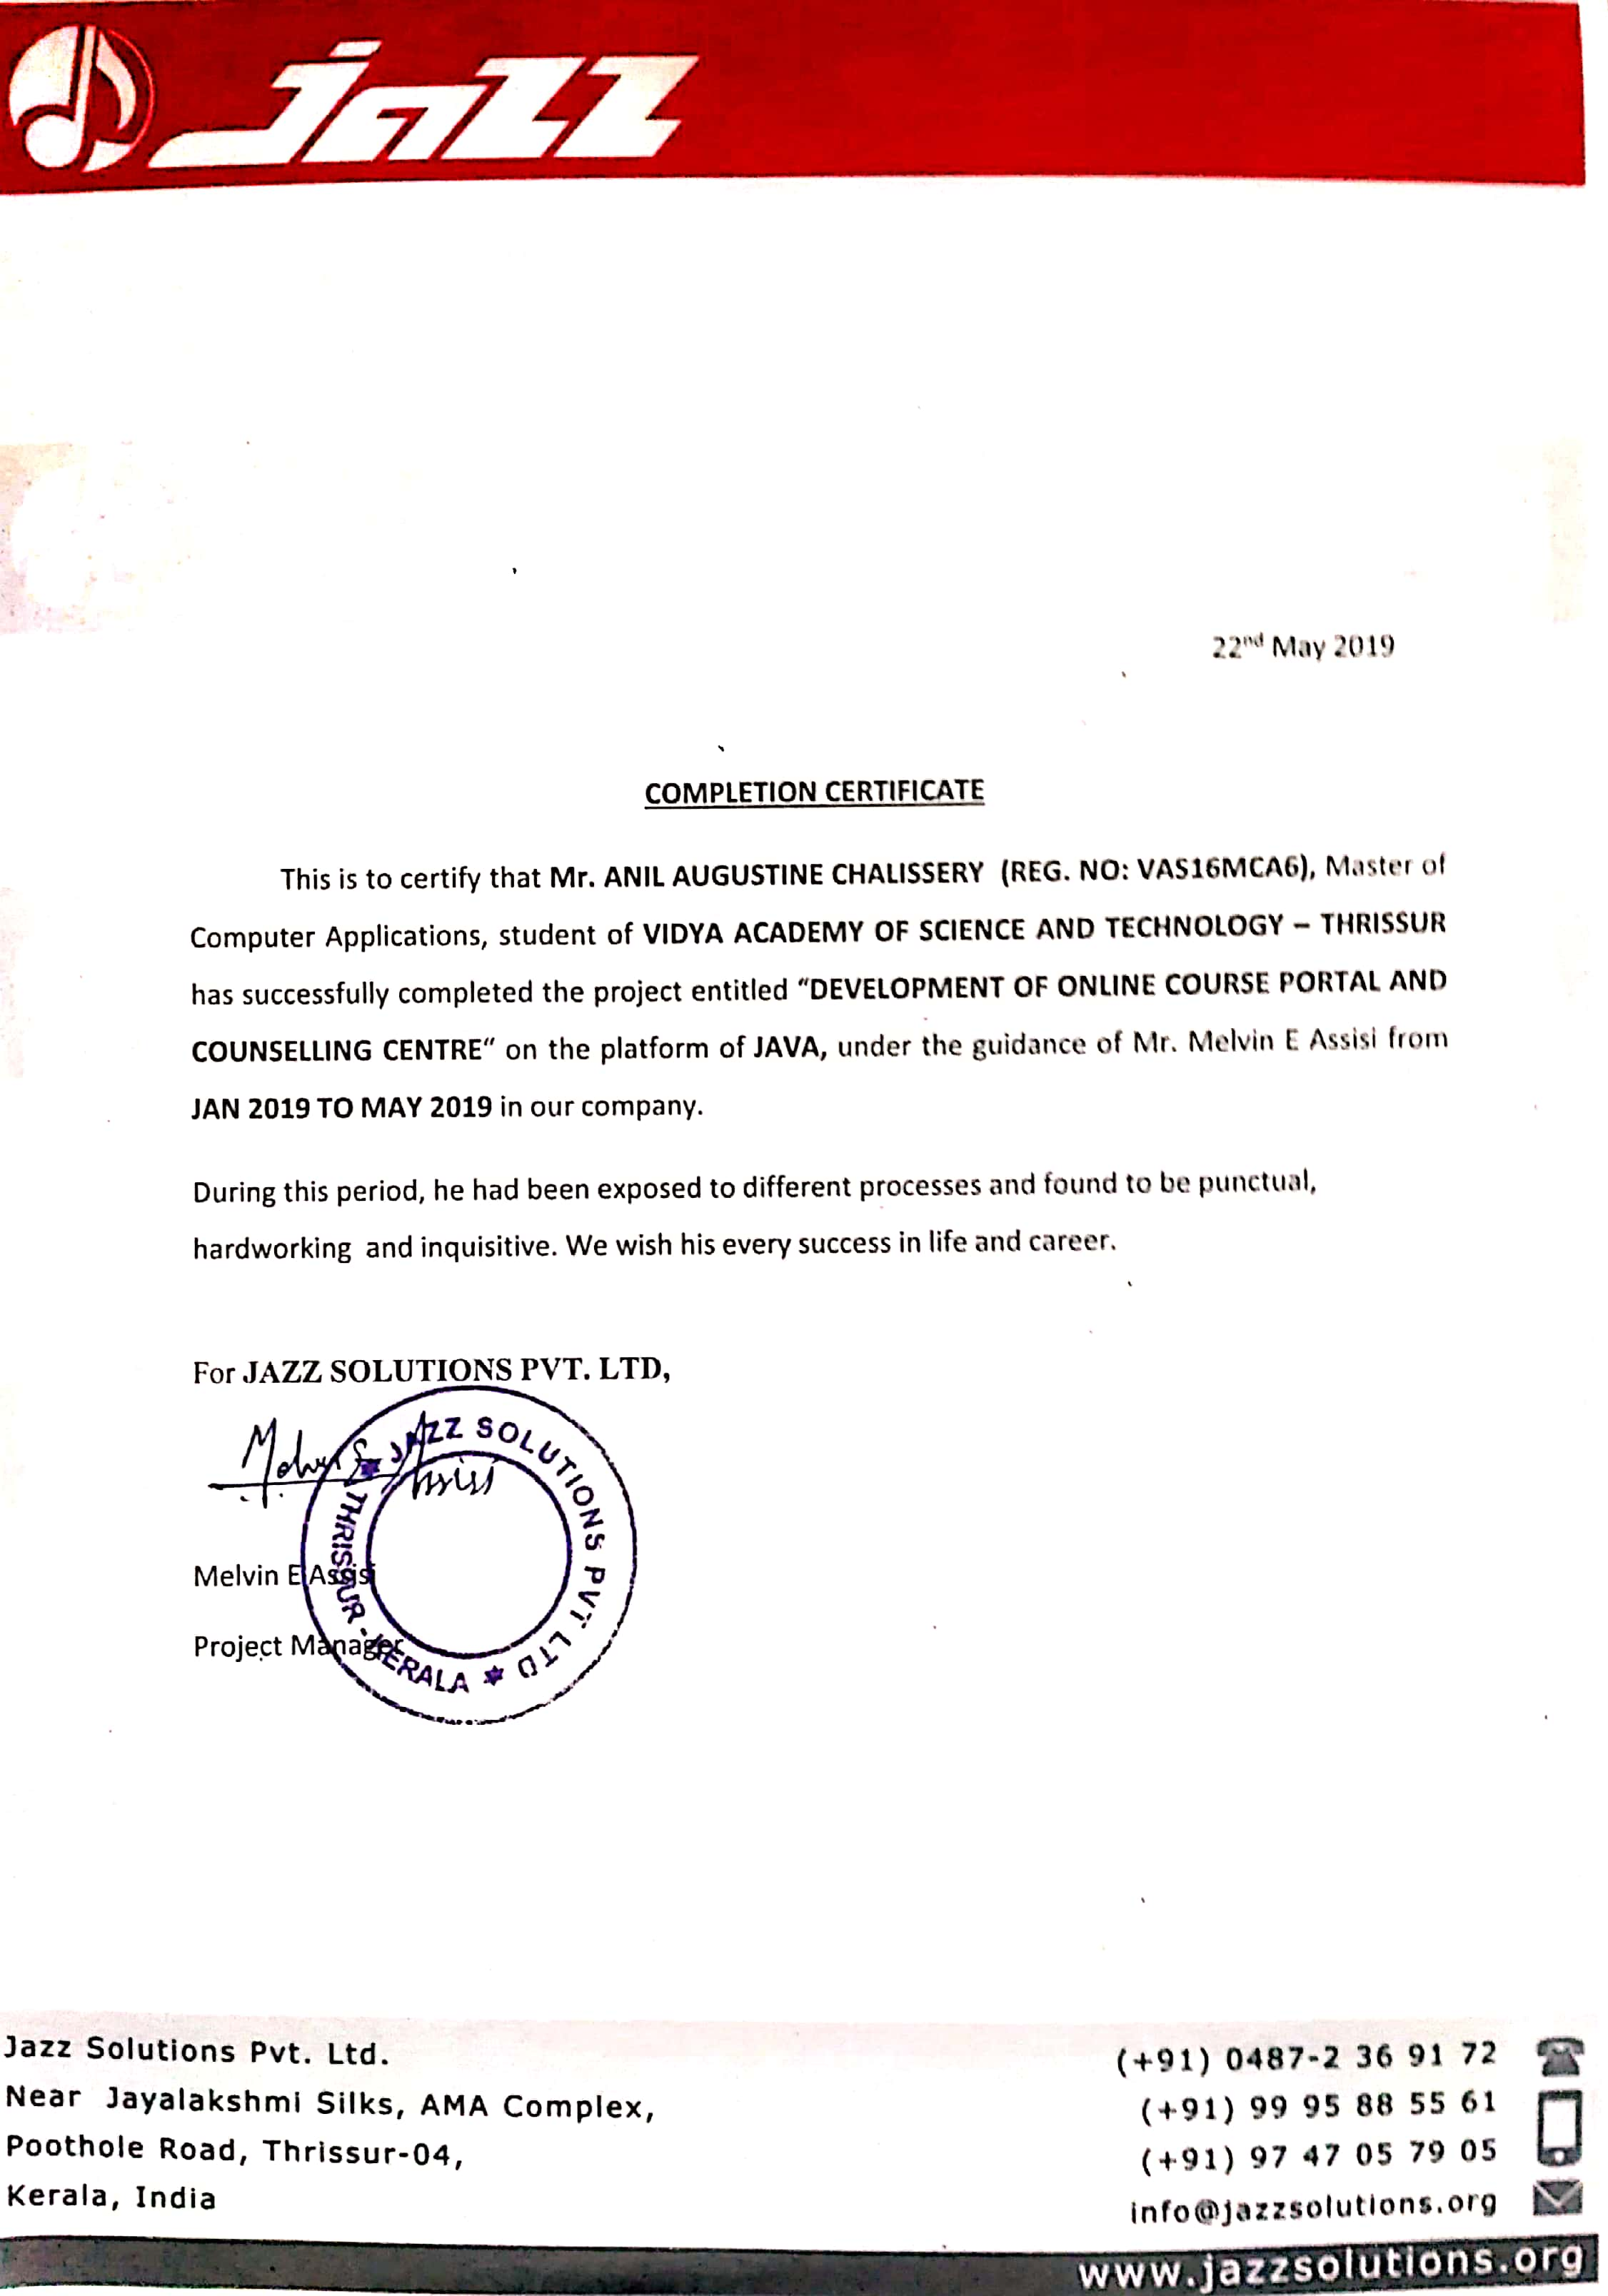
\includegraphics[height=\paperheight-0.75in, width= \paperwidth-0.75in]{certificatee}
\restoregeometry
\newpage
%
\clearpage
%
\addcontentsline{toc}{chapter}{Certificate from College}
%
\vspace*{\fill}
\pagestyle{plain}
\begin{center}
%
%
%   Department particulars
%
{\Large \bf Department of Computer Applications \par  }%\\[0.2cm]
{\large \bf Vidya Academy of Science \& Technology\par}%\\
{\normalsize \bf Thalakkottukara, Thrissur - 680 501\\
({\tt http://www.vidyaacademy.ac.in})\par}
\qquad\\[0.5cm]
%
%   Logo
%

\includegraphics{VidyaLogo.JPG}\\[0.75cm]
%
{\Large \bf CERTIFICATE}\\[0.75cm]
%
\end{center}
%
%   Certificate statement
%
This is to certify that the report titled 
{\bf \vtitle} is a bona-fide record of the 
work related to the paper \vpaper\  done  by 
{\bf \vauthor\  
(Reg. No. \vregisternumber)}    of  \vclass\  
(\vadmissionyear\ admissions) class 
of Vidya Academy of Science \& Technology, 
Thrissur - 680501 in partial fulfillment of the 
requirement for the award of the Degree of Master of Computer Applications  of APJ Abdul Kalam Technological University. \\[0.1cm]
%
%   Spaces for signatures 
%
\begin{center}
\begin{tabular}{p{0.10\textwidth}p{0.35\textwidth}p{0.10\textwidth}p{0.35\textwidth}}
%
\multicolumn{2}{l}{\bf Guide/Supervisor}    
&\multicolumn{2}{l}{\bf Head of Department}   \\
%
Name & : \vguide    & Name & : \vhod \\
%
Signature&: ...........................................
\qquad\quad   & 
Signature&: ...........................................\\
%
Date &: \today    & Date &: \today \\
%
\end{tabular}
\\[0.75cm]
%
%   Space for seal of Department
%
{\small (Seal of Department of \vdept)}
\end{center} 
%
\vspace*{\fill}
%
%   End of Certificate
%  
\clearpage
%
\addcontentsline{toc}{chapter}{Declaration by Student}
\thispagestyle{empty}
\chapter*{Declaration}
%
I, {\bf \vauthor}, studying in Sixth Semester MCA (2016 admissions) class of Vidya Academy of Science \&\  Technology, Thrissur -- 680501,    hereby declare that the project report 
(``\vtitle'') submitted by me for
partial fulfillment of the requirements for the award of degree of Master of Computer Applications of
APJ Abdul Kalam Technological University, Kerala, is a bona fide work done by me
under supervision of \vguide. This submission represents my ideas in
my own words and where ideas or words of others have been included, I have adequately
and accurately cited and referenced the original sources. I also declare that I have
adhered to ethics of academic honesty and integrity and have not misrepresented or
fabricated any data or idea or fact or source in my submission. I understand that any
violation of the above will be a cause for disciplinary action by the institute and/or the
University and can also evoke penal action from the sources which have thus not been
properly cited or from whom proper permission has not been obtained. This report has
not been previously formed the basis for the award of any degree, diploma or similar title
of any other University. 

\qquad\\[1cm]
\begin{tabular}{p{0.05\textwidth}p{0.27\textwidth}p{0.21\textwidth}p{0.35\textwidth}}
%
Place&: Thrissur -- 680501\qquad & Signature of student &: ......................................\\
Date&: \today & Name of student       &: \vauthor
\end{tabular}
\clearpage
%
\addcontentsline{toc}{chapter}{Acknowledgment}
%
\chapter*{Acknowledgment}
%
\index{acknowledgment}
I wish to record my indebtedness and thankfulness 
to all who helped me prepare this Report\index{seminar report} titled 
\vtitle\  and present it in a satisfactory way. This Report is part of my work related to the paper \vpaper.

I am especially thankful to my 
guide and supervisor \vguide\  in the Department of \vdept\  
for giving me valuable suggestions and 
critical inputs in the preparation of this report. 
I am also thankful to \vhod, 
the Head of \vdept\  
for encouragement. 

My friends in my class have always been 
helpful and I am grateful to them for 
patiently listening to  my presentations on my work related  of the project. 

\begin{flushright}
\vauthor\\
Reg. No. \vregisternumber\\
\vclass\  (\vadmissionyear\  Admissions)\\
Vidya Academy of Science \& Technology\\
Thrissur -680 501.
\end{flushright}
%
\clearpage
%
%
%****************************************************
%
%   No changes in the next two non-comment lines. These
%   lines are intended to create the Synopsis page and 
%   to add the the item "Synopsis" to 
%   table of contents.
%
\chapter*{Synopsis}
\addcontentsline{toc}{chapter}{Synopsis}
%
%   Enter below a synopsis of the project report. 
%   The two lines given
%   are to be deleted before entering actual abstract.

Online course portal(OCP) is one of the very efficient and effective way of combining learning, testing and discussing on one platform. Different courses are available so that  the student can have maximum benefit. Students who are willing to study more can further explore their required courses. Here the standard courses are available.

OCP allow instructors to upload course information for easy student access.  OCP  provide accessible exchange of information between professors and students. If the department delivers a course asynchronously, degree candidates may view lectures and course materials, such as PowerPoint presentations and syllabi, at their leisure. Synchronous courses, however, require scheduled attendance through online chats or conferencing.

Learners submit  assessments through OCP by posting on discussion forums and submitting tasks through applicable links. To submit a research paper, for instance, a student using Blackboard could click on the particular assignment link to upload the finished product. Professors may provide feedback to the student through comments or email when using this LMS.

 On the basis of standard courses that  are available the student can appear the quizzes respectively.The quizzing facility available provides the students to test their knowledge and further does their self assessment. It is also possible to clear the doubts as the discussion facility open for all. Anyone can discuss in public and achieve the complete knowledge.For all the facilities available,appropriate method have been used i.e. JSP (JavaServer Pages) technology.So the project is flexible,simple,efficient,secure and it is quite familiar to all.


%
%***************************************************
%
%   The next line creates a Table of Contents. 
%   Do not delete this. There must be a Table of Contents.
%
\clearpage
\addcontentsline{toc}{chapter}{Table of Contents}
\tableofcontents
%
%   The next line creates a page containing a 
%   List of Tables. Delete it if there are no 
%   tables in your project report. 
%
\clearpage
\addcontentsline{toc}{chapter}{List of Tables}
\listoftables
%
%   The next line creates a page containing a 
%   List of Figures. Delete it if there are no 
%   figures in your project report.
%

\clearpage
\addcontentsline{toc}{chapter}{List of Figures}
\listoffigures
%
%***************************************************
%
\mainmatter
%
\clearpage
\quad\vfill
\begin{center}
{\Huge \bf PROJECT REPORT}
\end{center}
\vfill
\clearpage
%
%
%   The main contents of the paper begin here. 
% 
%
%   *********************  CHAPTER ***********************
%
%  
\chapter{INTRODUCTION}
%
\section{Project Overview}
Online course portal is software developed for student in schools, colleges and institutes to access online course material. This project aims at creating a Courses portal for a campus/organization. This allows registered users of the system to join a course available in the site and access the materials published for the course. People can register themselves as students of a course or Faculty for a course. It facilitates to access the information of a particular course. The information is provided by the teacher for a particular course. The purpose of developing software  is to computerized the tradition way of taking class.

In order to form a clear sketch of this project, here’s a brief introduction of the features and scope of Online Course Management System. This project consists of three sections which are inter-linked to each other. These section are:
\begin{itemize}
\item Administrator Section
\item Students Section
\item Instructor Section
\end{itemize}
Each of the above section has certain specific task to perform. Administrator section is for controlling administrative works such as verifying and approving account for  instructors, view curriculum and coding the subjects etc. So, Administrator section can be considered as skeleton section on which other section rely on.

Student section and Instructor section have been designed for students and instructors to log in to the account created by administrator and share information. Students can register with application and submit their home work. Whereas, Instructors can check students’ home works and assign grades for their work.
%
\section{Organization Profile}

Jazz IT Solution was established in 2011. Jazz IT Solutions is the training wing of Aumento Performers Solutions Pvt Ltd (An ISO 9001-2008 Certified Company ) with the main objective of promoting IT Education and practices across the Globe.


	It’s a fast growing IT Education Company which has maintained its leadership in imparting quality services. Training programs will help prepare you for employment opportunities through traditional Instructor Led Training, hands-on training, certification achievement, and interviewing preparation. Jazz IT programs designed to give you real-world workplace experience.


	Jazz IT Solution provides the best IT training in the industry, different courses, online training etc. Jazz IT Solutionsr also provide internship, academic project guidance, online training for BTech/BE (ECE, EEE, CSE, IT) , MCA, MSc , MTech, BCA , BSc , Diploma students in different streams like Electronics , Electrical , Computer Science , Information Technology etc.


	Jazz IT Solution provide guideline in different platform like PHP , Android , JAVA ,Embedded System , Digital Image Processing (DIP) , VLSI , NS2 (networking) etc.

We are happy to introduce our self (Jazz IT Solution) as one of the growing training and staffing consultant in Kerala. We provide technical guidance to Software and electronic professionals. We help Professionals and students for specialize their technical skills. We are not just trainers who just provide training and certificate for a technical skill. We make our trainees to suit for the technology.


Jazz IT Solution provide academic project guidance to professional students. Academic project is important section for all kind of professional courses like MTech and Btech. Futuro IT Solutions gives minor and major project guidance to the student of MCA, BTech Computer Science, BTech Electronics, BSC Computer Science, and Diploma students. We will train the technology and make them confident to do their project themselves. That makes them unique in all other Project guidance centers and training institutes in Kerala.


Jazz IT Solution training team is a team of highly talented professionals. They make technical experts rather than professionals. Our hard working team coupled with professionalism results in total efficiency and superior skills, which benefit our clients and trainees alike.
%
%
%   *********************  CHAPTER ***********************
%
%
\chapter{SYSTEM ANALYSIS}
 System Analysis refers to the process of examining a business situation with the intent of improving it through better procedures and methods. System analysis relates to shaping organizations, improving performance and achieving objectives for profitability and growth. 

The emphasis is on systems in action, the relationships among subsystems and their contribution to meeting a common goal. Looking at a system and determining how adequately it functions, the changes to be made and the quality of the output are parts of system analysis. 
%
\section{The Existing System}
Offline education has been a part of our education system for as long we can remember.

In the existing system, we can store all the record manually that require large manpower and place to store all the records
this system was carried out through a manual process.


It leads to following disadvantages.
\begin{itemize}
\item Maintenance of records is difficult
\item Chance of occurrence of errors
\item Involves large amount of paperwork
\item Slow updating and renewal of data 
\end{itemize}	
%< Describe your various components here >
\section{Proposed System}
The current challenges facing traditional colleges and universities — including higher tuition, budget cuts, and course shortages — cause many students to search for alternatives. With nearly three million students currently enrolled in fully online programs and six million taking at least one online course as part of their degree, online education has clearly become one of the most popular higher education alternatives. The continually improving reputation of online learning helped fuel its expansion, as initial skepticism faltered in the face of evidence showing that online learning can be just as effective as face-to-face education.


All of this means that students, from working professionals to recent high school graduates, find many reasons to take all or some of their courses online.

Automated To overcome the disadvantages of the existing system we proposed the online system.
The best technology learning tools such as  group chats, multimedia presentation and interactive software are used by us to provide online education.

Online course portal is one of the very efficient and effective way of combining learning, testing and discussing on one platform. Different courses are available so that  the student can have maximum benefit. Students who are willing to study more can further explore their required courses. Here the standard courses are available.

 On the basis of standard courses that  are available the student can appear the quizzes respectively.The quizzing facility available provides the students to test their knowledge and further does their self assessment. It is also possible to clear the doubts as the discussion facility open for all. Anyone can discuss in public and achieve the complete knowledge.For all the facilities available,appropriate method have been used i.e. JSP (JavaServer Pages) technology.So the project is flexible,simple,efficient,secure and it is quite familiar to all.

This application introduce all types of question papers and solutions regarding the course
It also provides an audio lecture for each subject.
The  following are the advantages of proposed system.
\begin{itemize}
\item The automated system is time-saving and better performance than the manual based system.
\item Students are encouraged to think critically and support their opinions.
\item It supports the learning style of both audio and visual learners
\item class time is not wasted.
\item Students who excel in online class develop a system for keeping track of upcoming online exams and assignments due dates.
\item There are no traffic jams, parking hassles are adverse weather conditions
\item it enables the students to access course materials and contributed to discussion boards.
\item Home comfort.
\item Cost savings.

\end{itemize}
%
%
%   *********************  CHAPTER ***********************
%
%
\chapter{FEASIBILITY STUDY}
Feasibility study is a test of the system proposal according to its workability, impact on the organization, ability to meet user and effective use of resources. The objective of feasibility study is not to solve the problem. But to acquire a sense of its scope. During this study, the problem definition is crystalized and benefits are estimated with greater detail at this stage. The result of feasibility study is a system formal proposal. This is simply a form of documenting or detailing the nature and scope of proposed solution. The key considerations involved in the feasibility analysis are technical, economic and operational.
%
\section{Technical Feasibility}
     Technical feasibility centres on the existing manual system and to what extent it can support the system. According to feasibility analysis procedure the technical feasibility of the system is analyzed and the technical requirements such is software facilities, procedure, inputs, are identified. It is also one of the important phases of the system development activities.
%
\section{Economical Feasibility}
 Economic analysis is most frequently used for evaluation of the effectiveness of the system. More commonly known as cost/benefit analysis the procedure is to determine the benefit and saving that are expected from a system and compare them with cost, decision is made to design and implement the system. This part of feasibility study gives the economic justification of the system.     
 
         The system being developed is economic with respect to School or Collage’s point of view. It is cost effective in the sense that has eliminated the paper work completely. The system is also time effective because the calculations are automated which are made at the end of the month or as per the user requirement. The result obtained contains minimum errors and are highly accurate as the data is required. 
%
\section{Operational Feasibility}
 This is performed to check whether the system is operationally feasible or not. Using command buttons throughout the application programs enhances operational feasibility. So maintenance and modification is found to be easier. This feasibility is dependent on human resources (software development team) and involves visualizing whether the software will operate after it is developed and be operative once it is installed.A network admin can himself do all things in this system.
%
\chapter{SYSTEM DESIGN }
System designing in terms of software engineering has its own value and importance in the system development process as a whole. To mention it may though seem as simple as anything or simply the design of systems, but in a broader sense it implies a systematic and rigorous approach to design such a system which fulfills all the practical aspects including flexibility, efficiency and security. Systems design is the process of defining the architecture, components, modules, interfaces, and data for a system to satisfy specified requirements. Systems design could be seen as the application of systems theory to product development.

The system design covers the following ,Reviews the current physical system,  Prepares output specifications, Prepares input specifications,  Prepares edit, security and control specifications,  Specifies the implementation plan,  Prepares a logical design walk through of the information flow, output, input, controls  and implementation plan. 
%
\section{Input Design}
The input design is the link between the information system and the user. It comprises the developing specification and procedures for data preparation and those steps are necessary to put transaction data in to a usable form for processing can be achieved by inspecting the computer to read data from a written or printed document or it can occur by having people keying the data directly into the system. The design of input focuses on controlling the amount of input required, controlling the errors, avoiding delay, avoiding extra steps and keeping the process simple. The input is designed in such a way so that it provides security and ease of use with retaining the privacy. Input Design considered the following things that are what data should be given as an input, how the data should be arranged or coded, dialog to guide theoperating personnel in providing input and methods for preparing input validations and steps to follow when error occur.
%
\section{Output Design}
A quality output is one, which meets the requirements of the end user and presents the information clearly. In any system results of processing are communicated to the users and to other system through outputs. In output design it is determined how the information is to be displaced for immediate need and also the hard copy output. It is the most important and direct source information to the user. Efficient and intelligent output design improves the system’s relationship to help user decision-making.

Designing computer output should proceed in an organized, well thought out manner; the right output must be developed while ensuring that each output element is designed so that people will find the system can use easily and effectively. When analysis design computer output, they should Identify the specific output that is needed to meet the requirements.
%
\section{Database Design}
In designing a database application you must set up not only the program‘s routines for maximum performance, but you must pay attention also to the physical layout of the data storage. A good database design does the following:

Provides minimum search times when locating specific records.

Stores the data in efficient manner possible to keep the database from growing too large.

Makes data updates as easy as possible.

It is flexible enough to allow inclusion of new functions required of the program. 
 

 Normalization is a process of converting a relation to a standard form. The process is used to handle the problems that can arise due to data redundancy i.e. repetition of data in the database, maintain data integrity as well as handling problems that can arise due to insertion, updating, deletion anomalies. Insertion anomaly: Inability to add data to the database due to absence of other data. Deletion anomaly: Unintended loss of data due to deletion of other data. Update anomaly: Data inconsistency resulting from data redundancy and partial update. Decomposing is the process of splitting relations into multiple relations to eliminate anomalies and maintain anomalies and maintain data integrity. To do this we use normal forms or rules for structuring relation. Normal Forms are the rules for structuring relations that eliminate anomalies. 
 Different normal forms are used in database.

\begin{itemize}
\item {\bf First Normal Form}

A relation is said to be in first normal form if the values in the relation are atomic for every attribute in the relation. By this we mean simply that no attribute value can be a set of values or, as it is sometimes expressed, a repeating group.
\end{itemize}


\begin{itemize}
\item {\bf Second Normal Form:}

 A relation is said to be in second Normal form is it is in first normal form and it should satisfy any one of the following rules.
\begin{enumerate}
\item Primary key is a not a composite primary key
 \item  No non key attributes are present. 
\item Every non key attribute is fully functionally dependent on full set of primary key. 
\end{enumerate}
\end{itemize}

\begin{itemize}
\item {\bf Third Normal Form}

A relation is said to be in third normal form if their exits no transitive dependencies. Transitive Dependency: If two non-key attributes depend on each other as well as on the primary key then they are said to be transitively dependent. The above normalization principles were applied to decompose the data in multiple tables thereby making the data to be maintained in a consistent state.

The database is implemented using a DBMS package. Each particular DBMS has unique characteristics and general technique for database design. The application stores the information relevant for processing to SQL database. This SQL database contains tables where each table corresponding to one particular type of information. Each piece of information in a table is called a field or column. A table also contains records, which is a set of field. These are primary key fields that are uniquely identifying a record in a table. There are also fields that contain primary key from another table called foreign key.
\end{itemize}

\begin{itemize}
\item {\bf Candidate Key}

 In the relational model, a candidate key of a relation variable is a set of attributes of that relation variable such that At all times it holds in the relation assigned to that variable that there are no two distinct tuples with the same values for these attributes and There is not a proper subset of this set of attributes for which (1) holds.
\end{itemize}

\begin{itemize}
\item {\bf  Primary key}

In relational database design, a unique key or primary key is a candidate key to uniquely identify each row in a table. A unique key or primary key comprises a single column or set of columns. No two distinct rows in a table can have the same value in those columns. Depending on its design, a table may have arbitrarily many unique keys but at most one primary key. A unique key must uniquely identify all possible rows that exist in a table and not only the currently existing rows. Examples are social security numbers, id of student, id of employee etc.
\end{itemize}

\begin{itemize}
\item {\bf  Foreign key}

 In the context of relational databases, a foreign key is a referential constraint between two tables. The foreign key identifies a column or a set of columns in another table. The columns in the referencing table must be the primary key or other candidate key in the referenced table. The values in one row of the referencing columns must occur in a single row in the referenced table. Thus a row in the referencing table cannot contain values that don‘t exist in the referenced table.
\end{itemize}


\begin{itemize}
\item {\bf  Candidate key}

Candidate keys are those keys which is candidate for primary key of a table. In simple words we can understand that such type of keys which full fill all the requirements of primary key which is not null and have unique records is a candidate for primary key. So thus type of key is known as candidate key. Every table must have at least one candidate key but at the same time can have several.
\end{itemize}

\begin{itemize}
\item {\bf  Composite key}

When we create keys on more than one column then that key is known as composite key. Like here we can take an example to understand this feature. I have a table Student which has two columns Sid and SrefNo and we make primary key on these two column. Then this key is known as composite key.
\end{itemize}


\begin{itemize}
\item {\bf  Alternate key}

If any table have more than one candidate key, then after choosing primary key from those candidate key, rest of candidate keys are known as an alternate key of  that table. Like here we can take a very simple example to understand the concept of alternate key. Suppose we have a table named Employee which has two columns EmpID and EmpMail, both have not null attributes and unique value. So both columns are treated as candidate key. Now we make EmpID as a primary key to that table then EmpMail is known as alternate key.
\end{itemize}

%
%
%   *********************  CHAPTER ***********************
%
%
\chapter{IMPLEMENTATION , TESTING AND VALIDATION}

\section{Implementation}

{\bf Login.jsp}
\begin{lstlisting}
<%-- 
    Document   : Login
    Created on : Mar 28, 2019, 3:36:15 PM
    Author     : test
--%>
<!doctype html>
<html lang="en" class="fullscreen-bg">

<head>
	<title>Login | Online Course Portal</title>
	<meta charset="utf-8">
	<meta http-equiv="X-UA-Compatible" content="IE=edge,chrome=1">
	<meta name="viewport" content="width=device-width, initial-scale=1.0, 
		maximum-scale=1.0, user-scalable=0">
	<!-- VENDOR CSS -->
	<link rel="stylesheet" href="assets/css/bootstrap.min.css">
	<link rel="stylesheet"
		 href="assets/vendor/font-awesome/css/font-awesome.min.css">
	<link rel="stylesheet" href="assets/vendor/linearicons/style.css">
	<!-- MAIN CSS -->
	<link rel="stylesheet" href="assets/css/main.css">
	<!-- FOR DEMO PURPOSES ONLY. You should remove this in your project -->
	<link rel="stylesheet" href="assets/css/demo.css">
	<!-- GOOGLE FONTS -->
	<link href="https://fonts.googleapis.com/css?
		family=Source+Sans+Pro:300,400,600,700" rel="stylesheet">
	<!-- ICONS -->
	<link rel="apple-touch-icon" sizes="76x76"
		 href="assets/img/apple-icon.png">
	<link rel="icon" type="image/png" sizes="96x96" 
		href="assets/img/favicon.png">
        <script>
history.pushState(null,document.title, location.href);
window.addEventListener('popstate',function(event))
{
    history.pushState(null,document.title,location.href);
    
});
</script>
</head>

<body >
	<!-- WRAPPER -->
	<div id="wrapper">
		<div class="vertical-align-wrap">
			<div class="vertical-align-middle">
				<div class="auth-box">
                                     <div class="left">
						
				<div class="content">
							
				</div>
			</div>
                   <div class="right">
		<div class="content">
			<div class="header">
			<div class="logo text-center">
				<img src="assets/img/logo.png" alt="OCP Logo">
			</div>
				<p class="lead">Login to your account</p>
			</div>
               <form class="form-auth-small" action="LoginAction.jsp" method="Post">
				<div class="form-group">
			<label for="signin-email" class="control-label sr-only" >Email</label>
               <input type="email" class="form-control" id="signin-email" 
				 placeholder="Email" name="email" required>
				</div>
			<div class="form-group">
		<label for="signin-password" class="control-label sr-only">Password</label>
                          <input type="password" class="form-control" id="signin-password"  
				placeholder="Password" name="password" required>
								</div>
					<div class="form-group clearfix">
						<label class="fancy-checkbox element-left">
							<input type="checkbox">
							<span>Remember me</span>
						</label>
					</div>
		<button type="submit" class="btn btn-primary btn-lg btn-block">LOGIN</button>
			<div class="bottom">
		<span class="helper-text" >
			<i class="fa fa-lock"></i> 
				<a href="#">Forgot password?</a>
		</span>
                      <span class="helper-text">
		<i class="lnr lnr-user"></i> 
			<a href="StudentRegs.jsp">New user / Register now</a>
		</span>
								</div>
							</form>
						</div>
					</div>
				</div>
			</div>
		</div>
	</div>
	<!-- END WRAPPER -->
</body>

</html>

\end{lstlisting}

{\bf LoginAction.jsp}
\begin{lstlisting}
<%-- 
    Document   : LoginAction
    Created on : Mar 28, 2019, 3:47:18 PM
    Author     : test
--%>

<%@page import="java.sql.ResultSet"%>
<%@page import="DAL.DBConnect"%>
<%@page contentType="text/html" pageEncoding="UTF-8"%>
<!DOCTYPE html>
<html>
    <head>
        <meta http-equiv="Content-Type" content="text/html; charset=UTF-8">
        <title>JSP Page</title>
        <%String email=request.getParameter("email");
        String password=request.getParameter("password");
            // out.print("Select * from admin where a_email='"+email+"' and a_password='"+password+"'");
       ResultSet rs = DAL.DBConnect.SelectData("Select * from admin where a_email='"+email+"' and a_password='"+password+"'");
       ResultSet rs1 = DAL.DBConnect.SelectData("Select * from student where s_email='"+email+"' and s_password='"+password+"'");
       ResultSet rs2 = DAL.DBConnect.SelectData("Select * from instructor where i_email='"+email+"' and i_password='"+password+"'");
       session.setAttribute("type", "" ); 
       if(rs.next())
        { 
        String dbemail=rs.getString("a_email");
        String dbpassword=rs.getString("a_password");
        String username=rs.getString("a_name");
     //   out.print("Select * from admin where a_email="+email+" and a_password="+password);
        if(email.equals(dbemail) && password.equals(dbpassword))
        {
            session.setAttribute("user",username );
             session.setAttribute("type", "admin" );
//THIS IS HOW WE DECLARE THE USER IN A SESSION
			response.sendRedirect("home.jsp"); //AND WE REDIRECTED TO LOGIN PAGE
			
           // response.sendRedirect("home.jsp");
        }
        
        }
        else 
        {
             out.print("Sorry, username or password error!");
             String msg="Sorry, username or password error!";
          %>  
<jsp:include page="Login.jsp"></jsp:include>  
<%  
        } 
        %>
        <% 
            if(rs1.next())
        { 
        String dbemail=rs1.getString("s_email");
        String dbpassword=rs1.getString("s_password");
        String username=rs1.getString("s_name");
        String s_id=rs1.getString("s_id");
     //   out.print("Select * from admin where a_email="+email+" and a_password="+password);
        if(email.equals(dbemail) && password.equals(dbpassword))
        {
            session.setAttribute("user",username );
            session.setAttribute("s_id", s_id ); 
            session.setAttribute("type", "student" );
            //THIS IS HOW WE DECLARE THE USER IN A SESSION
            response.sendRedirect("s_home.jsp"); //AND WE REDIRECTED TO LOGIN PAGE
			
           // response.sendRedirect("home.jsp");
        }
        
        }
        else 
        {
             out.print("Sorry, username or password error!");
             String msg="Sorry, username or password error!";
          %>  
<jsp:include page="Login.jsp"></jsp:include>  
<%  
        } 
        %>
             <% 
            if(rs2.next())
        { 
        String dbemail=rs2.getString("i_email");
        String i_id=rs2.getString("i_id");
        String dbpassword=rs2.getString("i_password");
        String username=rs2.getString("i_name");
        if(email.equals(dbemail) && password.equals(dbpassword))
        {
            session.setAttribute("user",username );//THIS IS HOW WE DECLARE THE USER IN A SESSION
            session.setAttribute("i_id", i_id ); 
            session.setAttribute("type", "instructor" );
	 response.sendRedirect("i_home.jsp"); //AND WE REDIRECTED TO LOGIN PAGE
			
           // response.sendRedirect("home.jsp");
        }
                }
        else 
        {
             out.print("Sorry, username or password error!");
             String msg="Sorry, username or password error!";
          %>  
<jsp:include page="Login.jsp"></jsp:include>  
<%  
        } 
        %>
    </head>
    <body>
        <h1>Hello World!</h1>
            </body>
</html>

\end{lstlisting}

{\bf StudentRegistration.jsp}
\begin{lstlisting}
<%-- 
    Document   : userReg
    Created on : Apr 10, 2019, 10:05:39 PM
    Author     : test
--%>
<!doctype html>
<html lang="en">

<head>
	<title>Insert student data table | Online Course Portal</title>
        
	<meta charset="utf-8">
	<meta http-equiv="X-UA-Compatible" content="IE=edge,chrome=1">
	<meta name="viewport" content="width=device-width, initial-scale=1.0, maximum-scale=1.0, user-scalable=0">
	<!-- VENDOR CSS -->
	<link rel="stylesheet" href="assets/vendor/bootstrap/css/bootstrap.min.css">
	<link rel="stylesheet" href="assets/vendor/font-awesome/css/font-awesome.min.css">
	<link rel="stylesheet" href="assets/vendor/linearicons/style.css">
	<!-- MAIN CSS -->
	<link rel="stylesheet" href="assets/css/main.css">
	<!-- FOR DEMO PURPOSES ONLY. You should remove this in your project -->
	<link rel="stylesheet" href="assets/css/demo.css">
	<!-- GOOGLE FONTS -->
	<link href="https://fonts.googleapis.com/css?family=Source+Sans+Pro:300,400,600,700" rel="stylesheet">
	<!-- ICONS -->
	<link rel="apple-touch-icon" sizes="76x76" href="assets/img/apple-icon.png">
	<link rel="icon" type="image/png" sizes="96x96" href="assets/img/favicon.png">
</head>

<body>
	<!-- WRAPPER -->
	<div id="wrapper">
		<!-- NAVBAR -->
		<nav class="navbar navbar-default navbar-fixed-top">
			<div class="brand">
				<a href="Login.jsp"><img src="assets/img/logo.png" alt="ocp Logo" class="img-responsive logo"></a>
			</div>
			<div class="container-fluid">
				<div class="navbar-btn">
					<button type="button" class="btn-toggle-fullwidth"><i class="lnr lnr-arrow-left-circle"></i></button>
				</div>
			<!--	<form class="navbar-form navbar-left">
					<div class="input-group">
						<input type="text" value="" class="form-control" placeholder="Search dashboard...">
						<span class="input-group-btn"><button type="button" class="btn btn-primary">Go</button></span>
					</div>
				</form>-->
				<!--<div class="navbar-btn navbar-btn-right">
					<a class="btn btn-success update-pro" href="https://www.themeineed.com/downloads/klorofil-pro-bootstrap-admin-dashboard-template/?utm_source=klorofil&utm_medium=template&utm_campaign=KlorofilPro" title="Upgrade to Pro" target="_blank"><i class="fa fa-rocket"></i> <span>UPGRADE TO PRO</span></a>
				</div>-->
				<div id="navbar-menu">
					<!--<ul class="nav navbar-nav navbar-right">
						<li class="dropdown">
							<a href="#" class="dropdown-toggle icon-menu" data-toggle="dropdown">
								<i class="lnr lnr-alarm"></i>
								<span class="badge bg-danger">5</span>
							</a>
							<ul class="dropdown-menu notifications">
								<li><a href="#" class="notification-item"><span class="dot bg-warning"></span>System space is almost full</a></li>
								<li><a href="#" class="notification-item"><span class="dot bg-danger"></span>You have 9 unfinished tasks</a></li>
								<li><a href="#" class="notification-item"><span class="dot bg-success"></span>Monthly report is available</a></li>
								<li><a href="#" class="notification-item"><span class="dot bg-warning"></span>Weekly meeting in 1 hour</a></li>
								<li><a href="#" class="notification-item"><span class="dot bg-success"></span>Your request has been approved</a></li>
								<li><a href="#" class="more">See all notifications</a></li>
							</ul>
						</li>-->
					<!--	<li class="dropdown">
							<a href="#" class="dropdown-toggle" data-toggle="dropdown"><i class="lnr lnr-question-circle"></i> <span>Help</span> <i class="icon-submenu lnr lnr-chevron-down"></i></a>
							<ul class="dropdown-menu">
								<li><a href="#">Basic Use</a></li>
								<li><a href="#">Working With Data</a></li>
								<li><a href="#">Security</a></li>
								<li><a href="#">Troubleshooting</a></li>
							</ul>
						</li>-->
						<!--<li class="dropdown">
							<a href="#" class="dropdown-toggle" data-toggle="dropdown"><img src="assets/img/user.png" class="img-circle" alt="Avatar"> <span><%//out.print(uid);%></span> <i class="icon-submenu lnr lnr-chevron-down"></i></a>
							<ul class="dropdown-menu">
								<li><a href="#"><i class="lnr lnr-user"></i> <span>My Profile</span></a></li>
								<li><a href="#"><i class="lnr lnr-envelope"></i> <span>Message</span></a></li>
								<li><a href="#"><i class="lnr lnr-cog"></i> <span>Settings</span></a></li>
								<li><a href="Logout.jsp"><i class="lnr lnr-exit"></i> <span>Logout</span></a></li>
							</ul>
						</li>-->
						<!-- <li>
							<a class="update-pro" href="https://www.themeineed.com/downloads/klorofil-pro-bootstrap-admin-dashboard-template/?utm_source=klorofil&utm_medium=template&utm_campaign=KlorofilPro" title="Upgrade to Pro" target="_blank"><i class="fa fa-rocket"></i> <span>UPGRADE TO PRO</span></a>
						</li> -->
					</ul>
				</div>
			</div>
		</nav>
		<!-- END NAVBAR -->
		<!-- LEFT SIDEBAR -->
		<div id="sidebar-nav" class="sidebar">
			<div class="sidebar-scroll">
				<nav>
					<ul class="nav">
						<li><a href="StudentRegs.jsp" class="active"><i class="lnr lnr-user"></i> <span>Student Registration</span></a></li>
					
						<li><a href="instructorRegs.jsp" class=""><i class="lnr lnr-user"></i> <span>Instructor Registration</span></a></li>
				                <!--<li><a href="studenttables.jsp" class=""><i class="lnr lnr-dice"></i>Student Table</a></li>
									<li><a href="instructortables.jsp" class=""><i class="lnr lnr-dice"></i>Instructor Table</a></li>
									<li><a href="courseoptedtable.jsp" class=""><i class="lnr lnr-dice"></i>Course opted Table</a></li>
                                                                        <li><a href="coursedatatable.jsp" class=""><i class="lnr lnr-dice"></i>Course Table</a></li>
                                                                        <li><a href="depttable.jsp" class=""><i class="lnr lnr-dice"></i>Departments table</a></li>
                                                                        <li><a href="intract.jsp" class=""><i class="lnr lnr-dice"></i>Chat table</a></li>-->
				
					</ul>
				</nav>
			</div>
		</div>
		<!-- END LEFT SIDEBAR -->
		<!-- MAIN -->
		<div class="main">
			<!-- MAIN CONTENT -->
			<div class="main-content">
				<div class="container-fluid">
					<h3 class="page-title"> Student Registration</h3>
					<div class="row">
						<div class="col-md-6">
							<!-- BUTTONS -->
							
							<!-- END BUTTONS -->
                                                        
							<!-- INPUTS -->
							<div class="panel">
								<div class="panel-heading">
									<h3 class="panel-title">Inputs</h3>
								</div>
								<div class="panel-body">
                                                                    <form action="studentregaction_1.jsp" method="post">
                                                                        <input type="text" class="form-control" placeholder="Name" name="s_name" required>
									<br>
                                                                        
									<label class="fancy-radio">
										<input name="gender" value="Male" type="radio" checked >
										<span><i></i>Male</span>
									</label>
									<label class="fancy-radio">
										<input name="gender" value="Female" type="radio"  >
										<span><i></i>Female</span>
									</label>
									<br>
                                                                        <input type="email" class="form-control" placeholder="Email" name="s_email" required>
									<br>
                                                                        <input type="text" class="form-control" pattern="[7-9]{1}[0-9]{9}" title="Enter valid Number " placeholder="Mobile" name="s_mob" required>
									<br>
                                                                        
									<input type="password" class="form-control" placeholder="password"  name="s_password" required>
									<br>
                                                                        <input type="submit" value="Register" class="btn btn-primary">
									<br>
                                                                        <%
                                                            if(request.getParameter("a")!=null)
                                                            {
                                                                %> <jsp:include page="emailAlert.jsp"></jsp:include> <%
                                                            }
                                                        
                                                        %>
								
								</div>
							</div>
							<!-- END INPUTS -->
							
						</div>
						
					</div>
				</div>
			</div>
			<!-- END MAIN CONTENT -->
		</div>
		<!-- END MAIN -->
		<div class="clearfix"></div>
		<footer>
			<div class="container-fluid">
				<p class="copyright">&copy; 2017 <a href="https://www.themeineed.com" target="_blank">Theme I Need</a>. All Rights Reserved.</p>
			</div>
		</footer>
	</div>
	<!-- END WRAPPER -->
	<!-- Javascript -->
	<script src="assets/vendor/jquery/jquery.min.js"></script>
	<script src="assets/vendor/bootstrap/js/bootstrap.min.js"></script>
	<script src="assets/vendor/jquery-slimscroll/jquery.slimscroll.min.js"></script>
	<script src="assets/scripts/klorofil-common.js"></script>
</body>

</html>

\end{lstlisting}

{\bf StudentRegistrationAction.jsp}
\begin{lstlisting}
<%-- 
    Document   : studentregaction
    Created on : Mar 7, 2019, 2:50:09 PM
    Author     : test
--%>

<%@page import="DAL.DBConnect"%>
<%@page import="java.sql.ResultSet"%>
<%@page contentType="text/html" pageEncoding="UTF-8"%>
<!DOCTYPE html>
<html>
    <head>
        <meta http-equiv="Content-Type" content="text/html; charset=UTF-8">
        <title>registration process</title>
        <%
            // String type = (String)session.getAttribute("type");
        String s_name=request.getParameter("s_name");
        String gender=request.getParameter("gender");
        String s_email=request.getParameter("s_email");
        String s_password=request.getParameter("s_password");
        //String s_password_check=request.getParameter("s_password_check");
        String s_mob=request.getParameter("s_mob");
       String status="Pending";
       ResultSet rs=DBConnect.SelectData("Select * from student where s_email='"+s_email+"' ");
       //int flag=0;
       
           if(rs.next())
           {
                 %> <jsp:include page="StudentRegs.jsp?a=emailExists"></jsp:include><%
           }
else{
       
         DAL.DBConnect.ExecuteQuery("insert into student (s_name,gender,s_mob,s_email,s_password) values ('"+s_name+"','"+gender+"','"+s_mob+"','"+s_email+"','"+s_password+"')");
         response.sendRedirect("Login.jsp");
	} 
        %>
    </head>
    <body>
        <h1>Registered</h1>
    </body>
</html>

\end{lstlisting}

{\bf InstructorRegistration.jsp}
\begin{lstlisting}
<%-- 
    Document   : instructorRegs
    Created on : Apr 16, 2019, 9:10:34 AM
    Author     : test
--%>
<!doctype html>
<html lang="en">

<head>
	<title>Insert instructor | Online Course Portal</title>
        
	<meta charset="utf-8">
	<meta http-equiv="X-UA-Compatible" content="IE=edge,chrome=1">
	<meta name="viewport" content="width=device-width, initial-scale=1.0, maximum-scale=1.0, user-scalable=0">
	<!-- VENDOR CSS -->
	<link rel="stylesheet" href="assets/vendor/bootstrap/css/bootstrap.min.css">
	<link rel="stylesheet" href="assets/vendor/font-awesome/css/font-awesome.min.css">
	<link rel="stylesheet" href="assets/vendor/linearicons/style.css">
	<!-- MAIN CSS -->
	<link rel="stylesheet" href="assets/css/main.css">
	<!-- FOR DEMO PURPOSES ONLY. You should remove this in your project -->
	<link rel="stylesheet" href="assets/css/demo.css">
	<!-- GOOGLE FONTS -->
	<link href="https://fonts.googleapis.com/css?family=Source+Sans+Pro:300,400,600,700" rel="stylesheet">
	<!-- ICONS -->
	<link rel="apple-touch-icon" sizes="76x76" href="assets/img/apple-icon.png">
	<link rel="icon" type="image/png" sizes="96x96" href="assets/img/favicon.png">
</head>

<body>
	<!-- WRAPPER -->
	<div id="wrapper">
		<!-- NAVBAR -->
		<nav class="navbar navbar-default navbar-fixed-top">
			<div class="brand">
				<a href="Login.jsp"><img src="assets/img/logo.png" alt="ocp Logo" class="img-responsive logo"></a>
			</div>
			<div class="container-fluid">
				<div class="navbar-btn">
					<button type="button" class="btn-toggle-fullwidth"><i class="lnr lnr-arrow-left-circle"></i></button>
				</div>
			</div>
		</nav>
		<!-- END NAVBAR -->
		<!-- LEFT SIDEBAR -->
		
<div id="sidebar-nav" class="sidebar">
			<div class="sidebar-scroll">
				<nav>
					<ul class="nav">
						<li><a href="StudentRegs.jsp" class=""><i class="lnr lnr-user"></i> <span>Student Registration</span></a></li>
					
						<li><a href="instructorRegs.jsp" class="active"><i class="lnr lnr-user"></i> <span>Instructor Registration</span></a></li>
				                
					</ul>
				</nav>
			</div>
		</div>



                
		<!-- END LEFT SIDEBAR -->
		<!-- MAIN -->
		<div class="main">
			<!-- MAIN CONTENT -->
			<div class="main-content">
				<div class="container-fluid">
                                    
					<h3 class="page-title">Instructor Registration</h3>
                                        
					<div class="row">
                                            
						<div class="col-md-6">
							
							<!-- INPUTS -->
							<div class="panel">
								<div class="panel-heading">
									<h3 class="panel-title">Inputs</h3>
								</div>
								<div class="panel-body">
									<form action="instructorregaction.jsp" method="post">
									<input type="text" class="form-control" placeholder="Name" name="i_name" pattern="[A-Z a-z]{1,32}" required>
									<br>
                                                                        <label class="fancy-radio">
										<input name="gender" value="Male" type="radio" checked >
										<span><i></i>Male</span>
									</label>
									<label class="fancy-radio">
										<input name="gender" value="Female" type="radio"  >
										<span><i></i>Female</span>
									</label>
                                                                        <br>
                                                                        <input type="text" class="form-control" placeholder="Mobile number" pattern="[7-9]{1}[0-9]{9}" title="Enter valid Number "name="i_mob" required>
									<br>
                                                                        <input type="email" class="form-control" placeholder="Email" name="i_email" required>
									<br>
                                                                        <input type="text" class="form-control" placeholder="Currently Working Institution" name="workinginstitution" required>
									<br>
                                                                        <input type="text" class="form-control" placeholder="work address" name="workaddress" required>
									<br>
									<input type="password" class="form-control" placeholder="password"  name="i_password" required>
									<br>
                                                                        <input type="submit" value="Register" class="btn btn-primary">
									<br>
								<%
                                                            if(request.getParameter("a")!=null)
                                                            {
                                                                  %> <jsp:include page="emailAlert.jsp"></jsp:include> <%
                                                            }
                                                        
                                                        %>
								</div>
							</div>
							<!-- END INPUTS -->
							
						</div>
						
					
				</div>
			</div>
			<!-- END MAIN CONTENT -->
		</div>
		<!-- END MAIN -->
		<div class="clearfix"></div>
		<footer>
			<div class="container-fluid">
				<p class="copyright">&copy; 2017 <a href="https://www.themeineed.com" target="_blank">Theme I Need</a>. All Rights Reserved.</p>
			</div>
		</footer>
	</div>
	<!-- END WRAPPER -->
	<!-- Javascript -->
	<script src="assets/vendor/jquery/jquery.min.js"></script>
	<script src="assets/vendor/bootstrap/js/bootstrap.min.js"></script>
	<script src="assets/vendor/jquery-slimscroll/jquery.slimscroll.min.js"></script>
	<script src="assets/scripts/klorofil-common.js"></script>
</body>

</html>

\end{lstlisting}

{\bf InstructorRegistrationAction.jsp}
\begin{lstlisting}
<%-- 
    Document   : instructorregaction
    Created on : Mar 7, 2019, 3:05:21 PM
    Author     : test
--%>

<%@page import="DAL.DBConnect"%>
<%@page import="java.sql.ResultSet"%>
<%@page contentType="text/html" pageEncoding="UTF-8"%>
<!DOCTYPE html>
<html>
    <head>
        <meta http-equiv="Content-Type" content="text/html; charset=UTF-8">
        <title>Instructor registration process</title>
        <%
        String i_name=request.getParameter("i_name");
        String gender=request.getParameter("gender");
        String i_mob=request.getParameter("i_mob");
        String i_email=request.getParameter("i_email");
        String i_password=request.getParameter("i_password");
       // String i_password_check=request.getParameter("i_password_check");
          
        
        if((String)session.getAttribute("type")!=null){
        String status="Pending";
        //out.print("name"+i_name+"email"+i_email+"password"+i_password);
        ResultSet rs=DBConnect.SelectData("select * from instructor where i_email='"+i_email+"'");
        if(rs.next())
           {
                 %> <jsp:include page="instructorRegs.jsp?a=emailExists"></jsp:include><%
           }
        else{
       

             DAL.DBConnect.ExecuteQuery("insert into instructor (i_name,gender,i_mob,i_email,i_password,status) values ('"+i_name+"','"+gender+"','"+i_mob+"','"+i_email+"','"+i_password+"','"+status+"')");
        session.setAttribute("msg","sucess");
         response.sendRedirect("instructortables.jsp");
            }
          }
else{
String status="Pending";
        //out.print("name"+i_name+"email"+i_email+"password"+i_password);
        ResultSet rs=DBConnect.SelectData("select * from instructor where i_email='"+i_email+"'");
        if(rs.next())
           {
                 %> <jsp:include page="instructorRegs.jsp?a=emailExists"></jsp:include><%
           }
else{
       

         DAL.DBConnect.ExecuteQuery("insert into instructor (i_name,gender,i_mob,i_email,i_password,status) values ('"+i_name+"','"+gender+"','"+i_mob+"','"+i_email+"','"+i_password+"','"+status+"')");
        session.setAttribute("msg","sucess");
         response.sendRedirect("Login.jsp");

}
}
        
/*try{
                                             
                                         
                                         
                                          if(type.equals("admin"))
                                         {
                                         // out.print(type+"2");
                                             session.setAttribute("msg","sucess");
                                             response.sendRedirect("instructortables.jsp");   
                                         }
                                         else
                                         {
                                             //session.setAttribute("msg","sucess");
                                        //     out.print(type+"3");
                                             response.sendRedirect("Login.jsp");
                                         }
}
catch(Exception e){
    out.print(type+"4");
out.print(e);
}*/
        %>
    </head>
    <body>
        <h1>ADD course</h1>
            
    </body>
</html>

\end{lstlisting}

{\bf LogOut.jsp}
\begin{lstlisting}
<%-- 
    Document   : Logout
    Created on : Mar 29, 2019, 12:09:23 PM
    Author     : test
--%>

<%@page contentType="text/html" pageEncoding="UTF-8"%>
<!DOCTYPE html>
<html>
    <head>
        <meta http-equiv="Content-Type" content="text/html; charset=UTF-8">
        <title>JSP Page</title>
        
    
<% session.invalidate();
 response.sendRedirect("Login.jsp");
%> <!-- HERE WE ARE INVALIDATE THE SESSION, SO THAT NO VALUES WILL BE PRESENT IN SESSION -->
		
	  <script>
history.pushState(null,document.title, location.href);
window.addEventListener('popstate',function(event))
{
    history.pushState(null,document.title,location.href);
    
});
</script>
    </head>
    <body>
        <h1>Hello World!</h1>
    </body>
</html>

\end{lstlisting}


{\bf CreateTest.jsp}
\begin{lstlisting}
<%-- 
    Document   : i_createQuestionpaper
    Created on : May 20, 2019, 10:56:26 AM
    Author     : test
--%>


<%@page import="DAL.DBConnect"%>
<%@page import="java.sql.ResultSet"%>
<!doctype html>
<html lang="en">

<head>
	<title>Insert Course  | Online Course Portal</title>
        <%
		//HERE WE GETTING THE ATTRIBUTE DECLARED IN VALIDATE.JSP AND CHECKING IF IT IS NULL, THE USER WILL BE REDIRECTED TO LOGIN PAGE
				String uid = (String)session.getAttribute("user");
				if (uid == null)
				{
		%><!-- NOT A VALID USER, IF THE USER TRIES TO EXECUTE LOGGED IN PAGE DIRECTLY, ACCESS IS RESTRICTED -->
					 <jsp:forward page="Login.jsp"/>
		<%	
				}
				
		%> 
	<meta charset="utf-8">
	<meta http-equiv="X-UA-Compatible" content="IE=edge,chrome=1">
	<meta name="viewport" content="width=device-width, initial-scale=1.0, maximum-scale=1.0, user-scalable=0">
	<!-- VENDOR CSS -->
	<link rel="stylesheet" href="assets/vendor/bootstrap/css/bootstrap.min.css">
	<link rel="stylesheet" href="assets/vendor/font-awesome/css/font-awesome.min.css">
	<link rel="stylesheet" href="assets/vendor/linearicons/style.css">
	<!-- MAIN CSS -->
	<link rel="stylesheet" href="assets/css/main.css">
	<!-- FOR DEMO PURPOSES ONLY. You should remove this in your project -->
	<link rel="stylesheet" href="assets/css/demo.css">
	<!-- GOOGLE FONTS -->
	<link href="https://fonts.googleapis.com/css?family=Source+Sans+Pro:300,400,600,700" rel="stylesheet">
	<!-- ICONS -->
	<link rel="apple-touch-icon" sizes="76x76" href="assets/img/apple-icon.png">
	<link rel="icon" type="image/png" sizes="96x96" href="assets/img/favicon.png">
</head>

<body>
	<!-- WRAPPER -->
	<div id="wrapper">
		<!-- NAVBAR -->
		<nav class="navbar navbar-default navbar-fixed-top">
			<div class="brand">
				<a href="home.jsp"><img src="assets/img/logo.png" alt="Klorofil Logo" class="img-responsive logo"></a>
			</div>
			<div class="container-fluid">
				<div class="navbar-btn">
					<button type="button" class="btn-toggle-fullwidth"><i class="lnr lnr-arrow-left-circle"></i></button>
				</div>
				<form class="navbar-form navbar-left">
					
				</form>
				<!--<div class="navbar-btn navbar-btn-right">
					<a class="btn btn-success update-pro" href="https://www.themeineed.com/downloads/klorofil-pro-bootstrap-admin-dashboard-template/?utm_source=klorofil&utm_medium=template&utm_campaign=KlorofilPro" title="Upgrade to Pro" target="_blank"><i class="fa fa-rocket"></i> <span>UPGRADE TO PRO</span></a>
				</div>-->
				<div id="navbar-menu">
					<ul class="nav navbar-nav navbar-right">
						
						<li class="dropdown">
							<a href="#" class="dropdown-toggle" data-toggle="dropdown"><img src="assets/img/user.png" class="img-circle" alt="Avatar"> <span><%out.print(uid);%></span> <i class="icon-submenu lnr lnr-chevron-down"></i></a>
							<ul class="dropdown-menu">
								<li><a href="#"><i class="lnr lnr-user"></i> <span>My Profile</span></a></li>
								<li><a href="#"><i class="lnr lnr-envelope"></i> <span>Message</span></a></li>
								<li><a href="#"><i class="lnr lnr-cog"></i> <span>Settings</span></a></li>
								<li><a href="Logout.jsp"><i class="lnr lnr-exit"></i> <span>Logout</span></a></li>
							</ul>
						</li>
						<!-- <li>
							<a class="update-pro" href="https://www.themeineed.com/downloads/klorofil-pro-bootstrap-admin-dashboard-template/?utm_source=klorofil&utm_medium=template&utm_campaign=KlorofilPro" title="Upgrade to Pro" target="_blank"><i class="fa fa-rocket"></i> <span>UPGRADE TO PRO</span></a>
						</li> -->
					</ul>
				</div>
			</div>
		</nav>
		<!-- END NAVBAR -->
		<!-- LEFT SIDEBAR -->
		<div id="sidebar-nav" class="sidebar">
			<div class="sidebar-scroll"><%String i_id = (String)session.getAttribute("i_id");
                    ResultSet rss=DBConnect.SelectData("select * from instructor where i_id="+i_id);
                    rss.next();
                    String status = rss.getString("status");
                    %>
				<nav>
					<ul class="nav">
						<li><a href="i_home.jsp" class=""><i class="lnr lnr-home"></i> <span>Dashboard</span></a></li>
                                                <li><a href="i_profile.jsp" class=""><i class="lnr lnr-user"></i>View Profile</a></li>
						<%if(status.equals("Approved")){%><li><a href="i_approveStudents.jsp" class=""><i class="lnr lnr-alarm"></i>Approve Registration</a></li>
				                
                                                <li><a href="i_addCourse.jsp" class="active"><i class="lnr lnr-file-add"></i>Add Course</a></li>
                                                <li><a href="i_viewcourses.jsp" class=""><i class="lnr lnr-enter"></i>View added Courses</a></li>
                                                <li><a href="i_viewStudents.jsp" class=""><i class="lnr lnr-users"></i>View Students</a></li>
                                              <!--  <li><a href="i_answer.jsp" class=""><i class="lnr lnr-bubble"></i>Answer Students</a></li>-->
                                                <li><a href="i_viewintracts.jsp" class=""><i class="lnr lnr-bubble"></i>Interacts</a></li>
						<% } %>
					</ul>
				</nav>
			</div>
		</div>
		<!-- END LEFT SIDEBAR -->
		<!-- MAIN -->
		<div class="main">
			<!-- MAIN CONTENT -->
			<div class="main-content">
				<div class="container-fluid">
					<h3 class="page-title">Add Course
                                        </h3>
					<div class="row">
						<div class="col-md-12">
							
							<!-- INPUTS -->
							<div class="panel">
								<div class="panel-heading">
									<h3 class="panel-title">Inputs</h3>
								</div>
								<div class="panel-body">
									<form action="i_prepareTest.jsp" method="post">
									
									<br>
                                                                 
                <div class="input-group">
										<select name="c_id" class="form-control"><%ResultSet rs8=DBConnect.SelectData("SELECT * FROM `course` WHERE i_id="+i_id);
                                                                            while(rs8.next()){%>
                            <option value="<%out.print(rs8.getString("c_id"));%>"><%out.print(rs8.getString("c_name"));%></option>
                <% }  %>        </select>
										
									</div>
                <br>
                                                                       
                                                                        <br>
                                                                        <input type="submit" value="Submit" class="btn btn-primary">
                                                                        </form>
								
								</div>
							</div>
							<!-- END INPUTS -->
						
						</div>
						
					</div>
				</div>
			</div>
			<!-- END MAIN CONTENT -->
		</div>
		<!-- END MAIN -->
		<div class="clearfix"></div>
		<footer>
			<div class="container-fluid">
				<p class="copyright">&copy; 2017 <a href="https://www.themeineed.com" target="_blank">Theme I Need</a>. All Rights Reserved.</p>
			</div>
		</footer>
	</div>
	<!-- END WRAPPER -->
	<!-- Javascript -->
	<script src="assets/vendor/jquery/jquery.min.js"></script>
	<script src="assets/vendor/bootstrap/js/bootstrap.min.js"></script>
	<script src="assets/vendor/jquery-slimscroll/jquery.slimscroll.min.js"></script>
	<script src="assets/scripts/klorofil-common.js"></script>
</body>

</html>

\end{lstlisting}

{\bf test.jsp}
\begin{lstlisting}
<%-- 
    Document   : s_Opt_course
    Created on : Apr 8, 2019, 4:29:05 PM
    Author     : test
--%>

<%@page import="DAL.DBConnect"%>
<%@page import="java.sql.ResultSet"%>
<!doctype html>
<html lang="en">

<head>
	<title>Update student data table | Online Course Portal</title>
        <%
		//HERE WE GETTING THE ATTRIBUTE DECLARED IN VALIDATE.JSP AND CHECKING IF IT IS NULL, THE USER WILL BE REDIRECTED TO LOGIN PAGE
				String uid = (String)session.getAttribute("user");
                                 String s_id = (String)session.getAttribute("s_id");
				if (uid == null)
				{
		%><!-- NOT A VALID USER, IF THE USER TRIES TO EXECUTE LOGGED IN PAGE DIRECTLY, ACCESS IS RESTRICTED -->
					 <jsp:forward page="Login.jsp"/>
		<%	
				}
				
		%> 
	<meta charset="utf-8">
	<meta http-equiv="X-UA-Compatible" content="IE=edge,chrome=1">
	<meta name="viewport" content="width=device-width, initial-scale=1.0, maximum-scale=1.0, user-scalable=0">
	<!-- VENDOR CSS -->
	<link rel="stylesheet" href="assets/vendor/bootstrap/css/bootstrap.min.css">
	<link rel="stylesheet" href="assets/vendor/font-awesome/css/font-awesome.min.css">
	<link rel="stylesheet" href="assets/vendor/linearicons/style.css">
	<!-- MAIN CSS -->
	<link rel="stylesheet" href="assets/css/main.css">
	<!-- FOR DEMO PURPOSES ONLY. You should remove this in your project -->
	<link rel="stylesheet" href="assets/css/demo.css">
	<!-- GOOGLE FONTS -->
	<link href="https://fonts.googleapis.com/css?family=Source+Sans+Pro:300,400,600,700" rel="stylesheet">
	<!-- ICONS -->
	<link rel="apple-touch-icon" sizes="76x76" href="assets/img/apple-icon.png">
	<link rel="icon" type="image/png" sizes="96x96" href="assets/img/favicon.png">
</head>

<body>
	<!-- WRAPPER -->
	<div id="wrapper">
		<!-- NAVBAR -->
		<nav class="navbar navbar-default navbar-fixed-top">
			<div class="brand">
				<a href="s_home.jsp"><img src="assets/img/logo.png" alt="ocp Logo" class="img-responsive logo"></a>
			</div>
			<div class="container-fluid">
				<div class="navbar-btn">
					<button type="button" class="btn-toggle-fullwidth"><i class="lnr lnr-arrow-left-circle"></i></button>
				</div>
				<form class="navbar-form navbar-left">
					<div class="input-group">
						<input type="text" value="" class="form-control" placeholder="Search dashboard...">
						<span class="input-group-btn"><button type="button" class="btn btn-primary">Go</button></span>
					</div>
				</form>
				
				<div id="navbar-menu">
					<ul class="nav navbar-nav navbar-right">
						<li class="dropdown">
							<a href="#" class="dropdown-toggle icon-menu" data-toggle="dropdown">
								<i class="lnr lnr-alarm"></i>
								<span class="badge bg-danger">5</span>
							</a>
							<ul class="dropdown-menu notifications">
								<li><a href="#" class="notification-item"><span class="dot bg-warning"></span>System space is almost full</a></li>
								<li><a href="#" class="notification-item"><span class="dot bg-danger"></span>You have 9 unfinished tasks</a></li>
								<li><a href="#" class="notification-item"><span class="dot bg-success"></span>Monthly report is available</a></li>
								<li><a href="#" class="notification-item"><span class="dot bg-warning"></span>Weekly meeting in 1 hour</a></li>
								<li><a href="#" class="notification-item"><span class="dot bg-success"></span>Your request has been approved</a></li>
								<li><a href="#" class="more">See all notifications</a></li>
							</ul>
						</li>
						<li class="dropdown">
							<a href="#" class="dropdown-toggle" data-toggle="dropdown"><i class="lnr lnr-question-circle"></i> <span>Help</span> <i class="icon-submenu lnr lnr-chevron-down"></i></a>
							<ul class="dropdown-menu">
								<li><a href="#">Basic Use</a></li>
								<li><a href="#">Working With Data</a></li>
								<li><a href="#">Security</a></li>
								<li><a href="#">Troubleshooting</a></li>
							</ul>
						</li>
						<li class="dropdown">
							<a href="#" class="dropdown-toggle" data-toggle="dropdown"><img src="assets/img/user.png" class="img-circle" alt="Avatar"> <span><%out.print(uid);%></span> <i class="icon-submenu lnr lnr-chevron-down"></i></a>
							<ul class="dropdown-menu">
								<li><a href="#"><i class="lnr lnr-user"></i> <span>My Profile</span></a></li>
								<li><a href="#"><i class="lnr lnr-envelope"></i> <span>Message</span></a></li>
								<li><a href="#"><i class="lnr lnr-cog"></i> <span>Settings</span></a></li>
								<li><a href="Logout.jsp"><i class="lnr lnr-exit"></i> <span>Logout</span></a></li>
							</ul>
						</li>
						
					</ul>
				</div>
			</div>
		</nav>
		<!-- END NAVBAR -->
		<!-- LEFT SIDEBAR -->
		<div id="sidebar-nav" class="sidebar">
			<div class="sidebar-scroll">
				<nav>
					<ul class="nav">
						<li><a href="s_home.jsp" class=""><i class="lnr lnr-home"></i> <span>Dashboard</span></a></li>
                                                 <li><a href="s_profile.jsp" class=""><i class="lnr lnr-user"></i>View Profile</a></li>
                                                 <li><a href="s_Opt_course.jsp" class="active"><i class="fa fa-search"></i>Opt Course</a></li>
                                                <li><a href="s_opted_courses.jsp" class=""><i class="fa fa-line-chart"></i>Opted Course</a></li>
                                                <li><a href="i_viewintracts.jsp" class=""><i class="lnr lnr-bubble"></i>Queries</a></li>
							
				
					</ul>
				</nav>
			</div>
		</div>
		<!-- END LEFT SIDEBAR -->
		<!-- MAIN -->
		<div class="main">
			<!-- MAIN CONTENT -->
			<div class="main-content">
				<div class="container-fluid">
					<h3 class="page-title">TEST BEGINS</h3>
                                          
					<div class="row">
						<div class="col-md-12">
							<!-- BUTTONS -->
							
							<!-- END BUTTONS -->
							<!-- INPUTS -->
							<div class="panel">
								<div class="panel-heading">
									<h3 class="panel-title"></h3>
								</div>
								<div class="panel-body">
                                                                   <form action="appeartestAction.jsp" method="POST">
                                                                     <%
                                                                     String c_id=request.getParameter("c_id");
                                                                     ResultSet rs= DBConnect.SelectData("SELECT * FROM `course` WHERE c_id="+c_id);
                                                                     rs.next();
                                                                     %>           
                                                                     <input type="text" class="form-control" value="<%out.print(rs.getString("c_name"));%>">           
                                                                      <br>
                                                                     <%ResultSet rs2=DBConnect.SelectData("SELECT * FROM `test` WHERE c_id="+c_id); 
                                                                     int i=1;
                                                                         while(rs2.next()){%>
                                                                           <br><input type="text" class="form-control" name="<%out.print(rs2.getString("test_id"));%>" value="<%out.print(rs2.getString("q_no")+". ");%><%out.print(rs2.getString("Question"));%>">               
                                                                         <br>  <input type="radio"  name="<%out.print(i);%>" value="1"><%out.print(rs2.getString("oa"));%>
                                                                           <input type="radio"  name="<%out.print(i);%>" value="2"><%out.print(rs2.getString("ob"));%>
                                                                           <input type="radio"  name="<%out.print(i);%>" value="3"><%out.print(rs2.getString("oc"));%>
                                                                           <input type="radio"  name="<%out.print(i);%>" value="4"><%out.print(rs2.getString("od"));%><br>
                                                                <%       i++;  }
                                                                             %>           
                                                                             <input type="hidden" name="noQ" value="<%out.print(i-1);%>">
                                                                             <input type="hidden" name="c_id" value="<%out.print(c_id);%>">
                                                                             <br><input type="Submit" class="btn btn-primary">
									
                                                                    </form>
								</div>
							</div>
							<!-- END INPUTS -->
							<!-- INPUT SIZING -->
							
							<!-- END INPUT SIZING -->
						</div>
						<div class="col-md-6">
							<!-- LABELS -->
							
							<!-- END LABELS -->
							<!-- PROGRESS BARS -->
							
							<!-- END PROGRESS BARS -->
							<!-- INPUT GROUPS -->
						
							<!-- END INPUT GROUPS -->
							<!-- ALERT MESSAGES -->
							
							<!-- END ALERT MESSAGES -->
						</div>
					</div>
				</div>
			</div>
			<!-- END MAIN CONTENT -->
		</div>
		<!-- END MAIN -->
		<div class="clearfix"></div>
		<footer>
			<div class="container-fluid">
				<p class="copyright">&copy; 2017 <a href="https://www.themeineed.com" target="_blank">Theme I Need</a>. All Rights Reserved.</p>
			</div>
		</footer>
	</div>
	<!-- END WRAPPER -->
	<!-- Javascript -->
	<script src="assets/vendor/jquery/jquery.min.js"></script>
	<script src="assets/vendor/bootstrap/js/bootstrap.min.js"></script>
	<script src="assets/vendor/jquery-slimscroll/jquery.slimscroll.min.js"></script>
	<script src="assets/scripts/klorofil-common.js"></script>
</body>

</html>

\end{lstlisting}

{\bf testAction}
\begin{lstlisting}
<%-- 
    Document   : appeartestAction
    Created on : May 21, 2019, 11:05:15 AM
    Author     : test
--%>
<%@page import="DAL.DBConnect"%>
<%@page import="java.sql.ResultSet"%>
<%
String snoQ=request.getParameter("noQ");
String s_id=(String)session.getAttribute("s_id");
int noQ=Integer.parseInt(snoQ);
int i=1;
int count=0;
String c_id=request.getParameter("c_id");
ResultSet rs=DBConnect.SelectData("select * from test where c_id="+c_id);
while(noQ!=i){
    String res=request.getParameter(String.valueOf(i));
    
    while(rs.next()){
        if(rs.getString("answer").equals(res)){
            count++;
        }
            
    }
    i++;
}
//DAL.DBConnect.ExecuteQuery("INSERT INTO `testresults`( `s_id`, `c_id`, `score`) VALUES ('"+s_id+"','"+c_id+"','"+count+"')");
out.print("INSERT INTO `testresults`( `s_id`, `c_id`, `score`) VALUES ('"+s_id+"','"+c_id+"','"+count+"')");


%>
\end{lstlisting}

{\bf OptCourse.jsp}
\begin{verbatim}
<%-- 
    Document   : s_Opt_course
    Created on : Apr 8, 2019, 4:29:05 PM
    Author     : test
--%>

<%@page import="java.sql.ResultSet"%>
<!doctype html>
<html lang="en">

<head>
	<title>Update student data table | Online Course Portal</title>
        <%
		//HERE WE GETTING THE ATTRIBUTE DECLARED IN VALIDATE.JSP AND CHECKING IF IT IS NULL, THE USER WILL BE REDIRECTED TO LOGIN PAGE
				String uid = (String)session.getAttribute("user");
                                 String s_id = (String)session.getAttribute("s_id");
				if (uid == null)
				{
		%><!-- NOT A VALID USER, IF THE USER TRIES TO EXECUTE LOGGED IN PAGE DIRECTLY, ACCESS IS RESTRICTED -->
					 <jsp:forward page="Login.jsp"/>
		<%	
				}
				
		%> 
	<meta charset="utf-8">
	<meta http-equiv="X-UA-Compatible" content="IE=edge,chrome=1">
	<meta name="viewport" content="width=device-width, initial-scale=1.0, maximum-scale=1.0, user-scalable=0">
	<!-- VENDOR CSS -->
	<link rel="stylesheet" href="assets/vendor/bootstrap/css/bootstrap.min.css">
	<link rel="stylesheet" href="assets/vendor/font-awesome/css/font-awesome.min.css">
	<link rel="stylesheet" href="assets/vendor/linearicons/style.css">
	<!-- MAIN CSS -->
	<link rel="stylesheet" href="assets/css/main.css">
	<!-- FOR DEMO PURPOSES ONLY. You should remove this in your project -->
	<link rel="stylesheet" href="assets/css/demo.css">
	<!-- GOOGLE FONTS -->
	<link href="https://fonts.googleapis.com/css?family=Source+Sans+Pro:300,400,600,700" rel="stylesheet">
	<!-- ICONS -->
	<link rel="apple-touch-icon" sizes="76x76" href="assets/img/apple-icon.png">
	<link rel="icon" type="image/png" sizes="96x96" href="assets/img/favicon.png">
</head>

<body>
	<!-- WRAPPER -->
	<div id="wrapper">
		<!-- NAVBAR -->
		<nav class="navbar navbar-default navbar-fixed-top">
			<div class="brand">
				<a href="s_home.jsp"><img src="assets/img/logo.png" alt="ocp Logo" class="img-responsive logo"></a>
			</div>
			<div class="container-fluid">
				<div class="navbar-btn">
					<button type="button" class="btn-toggle-fullwidth"><i class="lnr lnr-arrow-left-circle"></i></button>
				</div>
				<form class="navbar-form navbar-left">
					<div class="input-group">
						<input type="text" value="" class="form-control" placeholder="Search dashboard...">
						<span class="input-group-btn"><button type="button" class="btn btn-primary">Go</button></span>
					</div>
				</form>
				
				<div id="navbar-menu">
					<ul class="nav navbar-nav navbar-right">
						<li class="dropdown">
							<a href="#" class="dropdown-toggle icon-menu" data-toggle="dropdown">
								<i class="lnr lnr-alarm"></i>
								<span class="badge bg-danger">5</span>
							</a>
							<ul class="dropdown-menu notifications">
								<li><a href="#" class="notification-item"><span class="dot bg-warning"></span>System space is almost full</a></li>
								<li><a href="#" class="notification-item"><span class="dot bg-danger"></span>You have 9 unfinished tasks</a></li>
								<li><a href="#" class="notification-item"><span class="dot bg-success"></span>Monthly report is available</a></li>
								<li><a href="#" class="notification-item"><span class="dot bg-warning"></span>Weekly meeting in 1 hour</a></li>
								<li><a href="#" class="notification-item"><span class="dot bg-success"></span>Your request has been approved</a></li>
								<li><a href="#" class="more">See all notifications</a></li>
							</ul>
						</li>
						<li class="dropdown">
							<a href="#" class="dropdown-toggle" data-toggle="dropdown"><i class="lnr lnr-question-circle"></i> <span>Help</span> <i class="icon-submenu lnr lnr-chevron-down"></i></a>
							<ul class="dropdown-menu">
								<li><a href="#">Basic Use</a></li>
								<li><a href="#">Working With Data</a></li>
								<li><a href="#">Security</a></li>
								<li><a href="#">Troubleshooting</a></li>
							</ul>
						</li>
						<li class="dropdown">
							<a href="#" class="dropdown-toggle" data-toggle="dropdown"><img src="assets/img/user.png" class="img-circle" alt="Avatar"> <span><%out.print(uid);%></span> <i class="icon-submenu lnr lnr-chevron-down"></i></a>
							<ul class="dropdown-menu">
								<li><a href="#"><i class="lnr lnr-user"></i> <span>My Profile</span></a></li>
								<li><a href="#"><i class="lnr lnr-envelope"></i> <span>Message</span></a></li>
								<li><a href="#"><i class="lnr lnr-cog"></i> <span>Settings</span></a></li>
								<li><a href="Logout.jsp"><i class="lnr lnr-exit"></i> <span>Logout</span></a></li>
							</ul>
						</li>
						
					</ul>
				</div>
			</div>
		</nav>
		<!-- END NAVBAR -->
		<!-- LEFT SIDEBAR -->
		<div id="sidebar-nav" class="sidebar">
			<div class="sidebar-scroll">
				<nav>
					<ul class="nav">
						<li><a href="s_home.jsp" class=""><i class="lnr lnr-home"></i> <span>Dashboard</span></a></li>
                                                 <li><a href="s_profile.jsp" class=""><i class="lnr lnr-user"></i>View Profile</a></li>
                                                 <li><a href="s_Opt_course.jsp" class="active"><i class="fa fa-search"></i>Opt Course</a></li>
                                                <li><a href="s_opted_courses.jsp" class=""><i class="fa fa-line-chart"></i>Opted Course</a></li>
                                                <li><a href="i_viewintracts.jsp" class=""><i class="lnr lnr-bubble"></i>Queries</a></li>
							
				
					</ul>
				</nav>
			</div>
		</div>
		<!-- END LEFT SIDEBAR -->
		<!-- MAIN -->
		<div class="main">
			<!-- MAIN CONTENT -->
			<div class="main-content">
				<div class="container-fluid">
					<h3 class="page-title">Apply for Course</h3>
                                          <% 
                                             try
                                             {
                                             String msg1 = (String)session.getAttribute("msg1");
                                         if(msg1.equals("failed"))
                                         {
                                        %>   <%@ include file = "warningalert.jsp" %>
                                        <% }
}
catch(Exception e){

}
                                         %>
					<div class="row">
						<div class="col-md-12">
							<!-- BUTTONS -->
							
							<!-- END BUTTONS -->
							<!-- INPUTS -->
							<div class="panel">
								<div class="panel-heading">
									<h3 class="panel-title"></h3>
								</div>
								<div class="panel-body">
                                                                   <form action="course_optingAction.jsp" method="POST">
                                                                                
                                                                                
                                                                                
                                                                                
                                                                           <table class="table table-striped">
										<thead>
											<tr>
												<th>sl no.</th>
												<th>course name</th>
                                                                                                <th>about course</th>
                                                                                                 <th>instructor_name</th>
                                                                                                  <th>duration</th>
                                                                                                   <th>department</th>
                                                                                                
											</tr>
										</thead>
										<tbody>
										<%
                                                                                    ResultSet rs=DAL.DBConnect.SelectData("SELECT * FROM `course`");
                                                                                    ResultSet rs1=DAL.DBConnect.SelectData("SELECT * FROM course INNER JOIN instructor on course.i_id=instructor.i_id");
                                                                                    int i=1;
                                                                                            while(rs.next()&&rs1.next()){
                                                                                    %>
                                                                                    <tr>
                                                                                        <td><%out.print(i);i++;%></td>
                                                                                        <td><%out.print(rs.getString("c_name"));%></td>
                                                                                        <td><%out.print(rs.getString("about_course"));%></td>
                                                                                        <td><%out.print(rs1.getString("i_name"));%></td>
                                                                                        <td><%out.print(rs.getString("duration"));%></td>
                                                                                        <td><%out.print(rs.getString("dept"));%></td>
                                                                                            
                                                                                             
                                                                                             <td><a href=course_optingAction.jsp?s_id=<%out.print(s_id);%>&c_id=<%out.print(rs.getString("c_id"));%> class="btn btn-primary">Register</a></td>
                                                                                            <!-- <td><a href=deletecoursedata.jsp?c_id=<%//out.print(rs.getString("c_id"));%> class="btn btn-danger">delete</a></td>-->
                                                                                    </tr>
                                                                                    <% } %>
										</tbody>
									</table>     
                                                                                	
                                                                    </form>
								</div>
							</div>
							<!-- END INPUTS -->
							
						</div>
						
					</div>
				</div>
			</div>
			<!-- END MAIN CONTENT -->
		</div>
		<!-- END MAIN -->
		<div class="clearfix"></div>
		<footer>
			<div class="container-fluid">
				<p class="copyright">&copy; 2017 <a href="https://www.themeineed.com" target="_blank">Theme I Need</a>. All Rights Reserved.</p>
			</div>
		</footer>
	</div>
	<!-- END WRAPPER -->
	<!-- Javascript -->
	<script src="assets/vendor/jquery/jquery.min.js"></script>
	<script src="assets/vendor/bootstrap/js/bootstrap.min.js"></script>
	<script src="assets/vendor/jquery-slimscroll/jquery.slimscroll.min.js"></script>
	<script src="assets/scripts/klorofil-common.js"></script>
</body>

</html>

\end{verbatim}

{\bf OptCourseAction.jsp}
\begin{lstlisting}
<%-- 
    Document   : course_optingAction
    Created on : Mar 11, 2019, 2:24:47 PM
    Author     : test
--%>

<%@page import="java.sql.ResultSet"%>
<%@page contentType="text/html" pageEncoding="UTF-8"%>
<!DOCTYPE html>
<html>
    <head>
        <meta http-equiv="Content-Type" content="text/html; charset=UTF-8">
        <title>course opting</title>
    </head>
    <body>
        <h1></h1>
        <%
       // String c_id=request.getParameter("c_id");
        String s_id=request.getParameter("s_id");
        String c_id=request.getParameter("c_id");
        String status="Pending";
        ResultSet rs = DAL.DBConnect.SelectData("SELECT * FROM `course_opted` INNER JOIN course on course_opted.c_id=course.c_id where course.c_id="+c_id+" and course_opted.s_id="+s_id);
        if(!rs.next())
        {
        DAL.DBConnect.ExecuteQuery("INSERT INTO `course_opted`(`s_id`, `c_id`, `status`) VALUES ('"+s_id+"','"+c_id+"','"+status+"')");
        response.sendRedirect("s_opted_courses.jsp");
        session.setAttribute("msg1", "sucess" );  
        }
        else
        {
        out.print("already opted this course");
         response.sendRedirect("s_Opt_course.jsp");
        session.setAttribute("msg1", "failed" );
        }
        
        
        %>
    </body>
</html>

\end{lstlisting}


{\bf mycourses.jsp}
\begin{lstlisting}
<%-- 
    Document   : mycourses
    Created on : Apr 13, 2019, 9:13:26 PM
    Author     : test
--%>
<%@page import="java.sql.ResultSet"%>

<div class="panel">
    <div class="panel-heading">
	<h3 class="panel-title">Courses</h3>
    </div>
<div class="panel-body">
    <table class="table table-striped">
	<thead>
            <tr>
		<th>sl no.</th>
		<th>course name</th>
                <th>Students</th>
            </tr>
        </thead>
        <tbody>
	<%ResultSet rs=DAL.DBConnect.SelectData("SELECT * FROM `course` where i_id="+i_id);
                                                                                 //   ResultSet rs1=DAL.DBConnect.SelectData("SELECT * FROM course INNER JOIN instructor on course.i_id=instructor.i_id");
             int i=1;
              while(rs.next()){
                  ResultSet rs1=DAL.DBConnect.SelectData("select count(s_id) from course_opted where c_id="+rs.getString("c_id"));
                  rs1.next();
                  %>
         <tr>
           <td><%out.print(i);i++;%></td>
           <td><%out.print(rs.getString("c_name"));%></td>
            <td><%out.print(rs1.getString("count(s_id)"));%></td>
         </tr>
                         <% } %>
	</tbody>
	</table>
	</div>
</div>
\end{lstlisting}
{\bf StudentProfile.jsp}
\begin{verbatim}
<%-- 
    Document   : s_profile
    Created on : Apr 8, 2019, 3:03:40 PM
    Author     : test
--%>
<%@page import="java.sql.ResultSet"%>
<!doctype html>
<html lang="en">

<head>
	<title>Student Tables | Online Course Portal</title>
        <%
		//HERE WE GETTING THE ATTRIBUTE DECLARED IN VALIDATE.JSP AND CHECKING IF IT IS NULL, THE USER WILL BE REDIRECTED TO LOGIN PAGE
				String uid = (String)session.getAttribute("user");
                                String s_id = (String)session.getAttribute("s_id");
				if (uid == null)
				{
		%><!-- NOT A VALID USER, IF THE USER TRIES TO EXECUTE LOGGED IN PAGE DIRECTLY, ACCESS IS RESTRICTED -->
					 <jsp:forward page="Login.jsp"/>
		<%	
				}
				
		%> 
	<meta charset="utf-8">
	<meta http-equiv="X-UA-Compatible" content="IE=edge,chrome=1">
	<meta name="viewport" content="width=device-width, initial-scale=1.0, maximum-scale=1.0, user-scalable=0">
	<!-- VENDOR CSS -->
	<link rel="stylesheet" href="assets/vendor/bootstrap/css/bootstrap.min.css">
	<link rel="stylesheet" href="assets/vendor/font-awesome/css/font-awesome.min.css">
	<link rel="stylesheet" href="assets/vendor/linearicons/style.css">
	<!-- MAIN CSS -->
	<link rel="stylesheet" href="assets/css/main.css">
	<!-- FOR DEMO PURPOSES ONLY. You should remove this in your project -->
	<link rel="stylesheet" href="assets/css/demo.css">
	<!-- GOOGLE FONTS -->
	<link href="https://fonts.googleapis.com/css?family=Source+Sans+Pro:300,400,600,700" rel="stylesheet">
	<!-- ICONS -->
	<link rel="apple-touch-icon" sizes="76x76" href="assets/img/apple-icon.png">
	<link rel="icon" type="image/png" sizes="96x96" href="assets/img/favicon.png">
</head>

<body>
	<!-- WRAPPER -->
	<div id="wrapper">
		<!-- NAVBAR -->
		<nav class="navbar navbar-default navbar-fixed-top">
			<div class="brand">
				<a href="s_home.jsp"><img src="assets/img/logo.png" alt="ocp Logo" class="img-responsive logo"></a>
			</div>
			<div class="container-fluid">
				<div class="navbar-btn">
					<button type="button" class="btn-toggle-fullwidth"><i class="lnr lnr-arrow-left-circle"></i></button>
				</div>
				<form class="navbar-form navbar-left">
					<div class="input-group">
						<input type="text" value="" class="form-control" placeholder="Search dashboard...">
						<span class="input-group-btn"><button type="button" class="btn btn-primary">Go</button></span>
					</div>
				</form>
			
				<div id="navbar-menu">
					<ul class="nav navbar-nav navbar-right">
						
						
						<li class="dropdown">
							<a href="#" class="dropdown-toggle" data-toggle="dropdown"><img src="assets/img/user1.png" class="img-circle" alt="Avatar"> <span><%out.print(uid);%></span> <i class="icon-submenu lnr lnr-chevron-down"></i></a>
							<ul class="dropdown-menu">
								<li><a href="s_profile.jsp"><i class="lnr lnr-user"></i> <span>My Profile</span></a></li>
								
								<li><a href="Logout.jsp"><i class="lnr lnr-exit"></i> <span>Logout</span></a></li>
							</ul>
						</li>
						
					</ul>
				</div>
			</div>
		</nav>
		<!-- END NAVBAR -->
		<!-- LEFT SIDEBAR -->
		<div id="sidebar-nav" class="sidebar">
			<div class="sidebar-scroll">
				<nav>
					<ul class="nav">
						<li><a href="s_home.jsp" class=""><i class="lnr lnr-home"></i> <span>Dashboard</span></a></li>
                                                 <li><a href="s_profile.jsp" class="active"><i class="lnr lnr-user"></i>View Profile</a></li>
                                                 <li><a href="s_Opt_course.jsp" class=""><i class="fa fa-search"></i>Opt Course</a></li>
                                                <li><a href="s_opted_courses.jsp" class=""><i class="fa fa-line-chart"></i>Opted Course</a></li>
                                                <li><a href="i_viewintracts.jsp" class=""><i class="lnr lnr-bubble"></i>Queries</a></li>
							
				
					</ul>
				</nav>
			</div>
		</div>
		<!-- END LEFT SIDEBAR -->
		<!-- MAIN -->
		<div class="main">
			<!-- MAIN CONTENT -->
			<div class="main-content">
				<div class="container-fluid">
					<div class="panel panel-profile">
						<div class="">
                                                    <% 
                                             try
                                             {
                                             String msg = (String)session.getAttribute("msg");
                                         if(msg.equals("sucess"))
                                         {
                                        %>   <%@ include file = "sucessalert.jsp" %>
                                        <% }
}
catch(Exception e){

}
                                         %>
							<!-- LEFT COLUMN -->
							<div class="profile-left">
								<!-- PROFILE HEADER -->
								<div class="profile-header">
									<div class="overlay"></div>
									<div class="profile-main"><% ResultSet rs1 = DAL.DBConnect.SelectData("SELECT * FROM `student` where s_id="+s_id);
                                                                                                        rs1.next();%>
										<img src="assets/img/user.png" class="img-circle" alt="Avatar">
										<h3 class="name"><%out.print(rs1.getString("s_name")); %></h3>
										<span class="online-status status-available">Available</span>
									</div>
									<div class="profile-stat">
										
									</div>
								</div> 
								<!-- END PROFILE HEADER -->
								<!-- PROFILE DETAIL -->
								<div class="profile-detail">
									<div class="profile-info">
                                                                            <!--<div class="text-left"> Basic Info</div> <div class="text-right"><a href=s_UpdateStudentData.jsp?s_id=<% out.print(rs1.getString("s_id")); %> class="lnr lnr-pencil"></a></div> -->
										<ul class="list-unstyled list-justify">
                                                                                    <li><b class="heading" >Basic Info</b> <span><div class="text-right"><a href=s_UpdateStudentData.jsp?s_id=<% out.print(rs1.getString("s_id")); %> class="lnr lnr-pencil"></a></span></li>
											<li>Gender <span><%out.print(rs1.getString("gender")); %></span></li>
                                                                                    <li>Mobile <span><%out.print(rs1.getString("s_mob")); %></span></li>
											<li>Email <span><%out.print(rs1.getString("s_email")); %></span></li>
                                                                                        <li>Password <span> <div class="text-center"><a href=s_changepasswd.jsp?s_id=<% out.print(rs1.getString("s_id")); %> class="btn btn-primary">Change Password</a></div></span></li>
											
										</ul>
									</div>
                                                                                       
									<div class="profile-info">
										<h4 class="heading">Social</h4>
										<ul class="list-inline social-icons">
											<li><a href="https://www.facebook.com/onlinecourses.ooo/" class="facebook-bg"><i class="fa fa-facebook"></i></a></li>
											<li><a href="https://twitter.com/crunchadeal?lang=en" class="twitter-bg"><i class="fa fa-twitter"></i></a></li>
											
											<li><a href="https://github.com/anilchalissery/OnlineCoursePortal" class="github-bg"><i class="fa fa-github"></i></a></li>
										</ul>
									</div>
                                                                        
									<div class="profile-info">
										<!--<h4 class="heading">About</h4>
										<p>Interactively fashion excellent information after distinctive outsourcing.</p>-->
									</div>
									
								</div>
								<!-- END PROFILE DETAIL -->
							</div>
							<!-- END LEFT COLUMN -->
							<!-- RIGHT COLUMN -->
							<div class="profile-right">
								<h4 class="heading">Opted Courses</h4>
                                                                <%@ include file = "optedcourses.jsp" %>
                                                                
						
							</div>
							<!-- END RIGHT COLUMN -->
						</div>
					</div>
				</div>
			</div>
			<!-- END MAIN CONTENT -->
		</div>
		<!-- END MAIN -->
		<div class="clearfix"></div>
		<footer>
			<div class="container-fluid">
				<p class="copyright">&copy; 2017 <a href="https://www.themeineed.com" target="_blank">Theme I Need</a>. All Rights Reserved.</p>
			</div>
		</footer>
	</div>
	<!-- END WRAPPER -->
	<!-- Javascript -->
	<script src="assets/vendor/jquery/jquery.min.js"></script>
	<script src="assets/vendor/bootstrap/js/bootstrap.min.js"></script>
	<script src="assets/vendor/jquery-slimscroll/jquery.slimscroll.min.js"></script>
	<script src="assets/scripts/klorofil-common.js"></script>
</body>

</html>

\end{verbatim}


{\bf DBConnect.java}
\begin{lstlisting}
/*
 * To change this license header, choose License Headers in Project Properties.
 * To change this template file, choose Tools | Templates
 * and open the template in the editor.
 */
package DAL;

import java.sql.Connection;
import java.sql.DriverManager;
import java.sql.ResultSet;
import java.sql.SQLException;
import java.sql.Statement;

/**
 *
 * @author Melvin
 */
public class DBConnect {
     static Connection con;
      public static int c_id=0;
	
     public static Connection Connect()
	{
 		
 			
		try
		{
			Class.forName("com.mysql.jdbc.Driver");	
			con = DriverManager.getConnection("jdbc:mysql://localhost:3306/ocp","root","");
                        System.out.println("connected ");
		}
		catch(Exception e)
		{
			System.out.println("class error");
                       
		}
		return con;
	}
        
        
        
       
       
         public static void  ExecuteQuery(String Query){
     try {
         Connection conn=Connect();
        Statement st=conn.createStatement();
       
            st.execute(Query);
        } catch (SQLException ex) {
            
            System.out.println(ex.toString());
            System.out.println(Query);
          System.out.println("Query Error");
        }
        
    }
         
           public static int  ExecuteQueryReturn(String Query){
               int PrimeNo =0;
            try {
                Connection conn=Connect();
               Statement st=conn.createStatement();
              PrimeNo = st.executeUpdate(Query, Statement.RETURN_GENERATED_KEYS);
                   
               } catch (SQLException ex) {

                   System.out.println(ex.toString());
                   System.out.println(Query);
                 System.out.println("Query Error");
               }
            return PrimeNo;
        
    }
    
    public static ResultSet  SelectData(String Query){
        
        ResultSet rs=null;
     try {
         Connection conn=Connect();
        Statement st=conn.createStatement();
       
           rs= st.executeQuery(Query);
        } catch (SQLException ex) {
            
            System.out.println(ex.toString());
          System.out.println("Query Error");
        }
     return rs;
        
    }
    
     public static String getDate(String Date ){
       
           
            String[] str=Date.split("/");
            String convertDate="20"+str[2]+"/"+str[1]+"/"+str[0];
            
           return convertDate;
       }
    
}

\end{lstlisting}

{\bf FileUpload.java}
\begin{lstlisting}
/*
 * To change this license header, choose License Headers in Project Properties.
 * To change this template file, choose Tools | Templates
 * and open the template in the editor.
 */
package com.fileupload;

import DAL.DBConnect;
import java.io.File;
import java.io.IOException;
import java.util.List;

import javax.servlet.ServletException;
import javax.servlet.http.HttpServlet;
import javax.servlet.http.HttpServletRequest;
import javax.servlet.http.HttpServletResponse;

import org.apache.commons.fileupload.FileItem;
import org.apache.commons.fileupload.FileItemFactory;
import org.apache.commons.fileupload.disk.DiskFileItemFactory;
import org.apache.commons.fileupload.servlet.ServletFileUpload;

public class UploadFile extends HttpServlet {
        private static final long serialVersionUID = 1L;
        private final String UPLOAD_DIRECTORY = "C:/Files/";

        protected void doPost(HttpServletRequest request,
                HttpServletResponse response) throws ServletException, IOException {
        boolean isMultipart = ServletFileUpload.isMultipartContent(request);

        // process only if its multipart content
        if (isMultipart) {
                // Create a factory for disk-based file items
                FileItemFactory factory = new DiskFileItemFactory();

                // Create a new file upload handler
                ServletFileUpload upload = new ServletFileUpload(factory);
                try {
                    // Parse the request
                    List<FileItem> multiparts = upload.parseRequest(request);

                   for (FileItem item : multiparts) {
                   if (!item.isFormField()) {
                   String name = new File(item.getName()).getName();
                   DAL.DBConnect.ExecuteQuery("update course set datafile='"+name+"' where c_id='"+DBConnect.c_id+"'");
                   item.write(new File(UPLOAD_DIRECTORY + File.separator + DBConnect.c_id + name));
                   }
                }
                        
                // File uploaded successfully
                request.setAttribute("message", "Your file has been uploaded!");
                } 
                catch (Exception e) 
                {
                 request.setAttribute("message", "File Upload Failed due to " + e);
                }
        } else 
        {
        request.setAttribute("message", "This Servlet only handles file upload request");
        }
        request.getRequestDispatcher("/i_viewcourses.jsp").forward(request, response);
}
}
\end{lstlisting}



%
\section{Testing Methods}

In system testing the behavior of whole system or product is tested as defined by the scope of the development project or product. It may include tests based on risks and/or requirement specifications, business process, use cases, or other high level descriptions of system behavior, interactions with the operating systems, and system resources. System testing is most often the final test to verify that the system to be delivered meets the specification and its purpose. System testing is carried out by specialist testers or independent testers. System testing should investigate both functional and non-functional requirements of the testing. 

{\bf5.1.1. Unit Testing}

 Unit testing is a software testing method by which individual units of source code, sets of one or more computer program modules together with associated control data, usage procedures, and operating procedures, are tested to determine whether they are fit for use. Intuitively, one can view a unit as the smallest testable part of an application. In procedural programming, a unit could be an entire module, but it is more commonly an individual function or procedure. This is one of the main level of testing included in the testing methods. In object-oriented programming, a unit is often an entire interface, such as a class, but could be an individual method. Unit tests are short code fragments created by programmers or occasionally by white box testers during the development process. It forms the basis for component testing. Ideally, each test case is independent from the others. Substitutes such as method stubs, mock objects, fakes, and test harnesses can be used to assist testing a module in isolation. Unit tests are typically written and run by software developers to ensure that code meets its design and behaves as intended. In this system each unit is tested separately before integrating them into modules to test the interfaces between modules. 

{\bf5.1.2. Integration Testing }

When the modules of the system are combined together to form the whole system, there will be the problem of interfacing. Integration testing is a systematic testing technique for constructing the program structure while conducting tests to uncover errors associated with interfacing. The current system modules are combining using bottom-up integration with incremental method. The modules like message, file and watermark are combined to form either embedding or retrieving. Our system, test the integrated modules. In which we test the related forms together to ensure their relationship. 

% < Describe the various Testing methods used here >
\section{Validation}

The definition for the validation testing is that the validation succeeds when software functions in a manner that can be reasonably expected by the customer. The expectations are defined in the software requirements specifications. Validation criteria: The number of characters in the password must contain minimum of four characters. The password will be treated as invalid when the number of characters in it is less than four. Our system, test whether the required fields are empty or not. This system ensure that the fields must be filled and also ensure the minimum range of some fields.

After performing the validation testing, the next step is output testing of the proposed system since no system could be useful if it does not produce the required output in the specific format. The output generated or displayed by the system under consideration is tested asking the users about the format required by then. Here, the output is considered into ways: one is on the screen and the other is printed format. The output format on the screen is found to be correct as the format designed according to the user needs. For the hard copy also, the output comes out as specified by the user. Hence output testing doesn’t result in any connection in the system.





%	< Validation done in the project >
%
%   *********************  CHAPTER ***********************
%
%
\chapter{SYSTEM SECURITY MEASURES}
\begin{enumerate}
\item {\bf Physical }

This site containing the computer systems is physically secured against arms or surreptitious entry by intruders. 

\item {\bf Operating System }

No matter how to secure the system is, weakness in operating system security may serves as a means of unauthorized access to the network. Here Windows 8.1 as an operating system provides better level of security.  

\item {\bf Network }

Since almost all network system allows remote access through terminals and networks, software –level security within the network software is important. Network security can be attained by setting firewall and security options available with windows.  

\item {\bf Database System }

           SQL Server database implementation provides better security to data from unauthorized data access from loss data. SQL Server has built in user management, encryption and restore facility. 


\item {\bf Correction}

Even with the best quality assurance activities, it is likely that the customer will uncover defects in the software. Corrective maintenance changes the software to correct defects. 

\item {\bf Password }

 Password is the main security system for our site. This authorization mechanism limits the interaction with the resources to collection of user or system for enforcing integrity, confidentiality or availability constraints. There will be secret password for the user of the system. Hence, authorized users cannot access data of the system.

\item {\bf Enhancement}

As the software is used, the user will recognize additional functions that will provide benefit. Perfective maintenance extends the software beyond its original functional requirements.


\item {\bf Adaptation }

Over time, the original environment (e.g. CPU, Operating System, Business Rules, and External Product Characteristics) for which was developed was likely to change. Adaptive maintenance results in the modification to the software to accommodate changes to its external environment.

\item {\bf System maintenance}

Computer based business systems are dynamic. They must be able to accommodate changes in the business environment. These changes occur not only during the study, design, and development phases of the life cycle of the system, but also throughout its operational life. Maintenance involves the software industry captive, typing up the system resources. It means restoring something to its original condition. Maintenance involves a wide range of activities including correcting, coding and design errors, updating documentation and test data and upgrading user support. Maintenance is continued till the product is re-engineered or deployed to another platform. Maintenance is also done based on fixing the problems reported, changing the interface with other software or hardware enhancing the software.Security measures are provided to prevent unauthorized access of the database at various levels. An uninterrupted power supply should be so that the power failure or voltage fluctuations will not erase the data in the files. 

We can define maintenance by fair different maintenance activities.
\begin {enumerate}
\item Corrective maintenance.
\item Adaptive maintenance.
\item Perfective maintenance or enhancement.
\item Preventive maintenance or reengineering.
\end{enumerate}

\item {\bf Prevention}

Computer software deteriorates due to change, and because of this, preventive maintenance, often called software reengineering, must be conducted to enable preventive maintenance makes changes to computer programs. So that they can be more easily corrected, adapted and enhanced.
\end{enumerate}
  
%
%
%   *********************  CHAPTER ***********************
%
%
\chapter{CONCLUSION}
Online course portal is one of the very efficient and effective way of combining learning, testing and discussing on one platform. Different courses are available so that  the student can have maximum benefit. Students who are willing to study more can further explore their required courses. 

On the basis of courses that  are available the student can appear the quizzes respectively. The quizzing facility available provides the students to test their knowledge and further does their self assessment. It is also possible to clear the doubts as the discussion facility open for all. Anyone can discuss in public and achieve the complete knowledge.

%
\chapter{SCOPE FOR FUTURE ENHANCEMENT}
In future since each and every application should expand and it should provide a way for updating the system has been developed. All modules in the system are being developed carefully. Such that the future enhancement does not affect the basic performance of the system.
\begin{enumerate}
 \item Generate temporary timetable for exam days.
\item Online Streaming Class
\item Alert the students in the case of substitution class.
\item Provide Assignments
\item International Hackthons
\item Oauth Facility for login 
\item Paid Services
\item Programing interfaces for programing courses
\end{enumerate}
Later we are also planning to develop this project as an android application. Also extending facility with notifying through SMS can also be applied for future scope.

%
%
%   *********************  CHAPTER ***********************
%
%%%%%%%%%%%%%%%%%%%%%%%%%  APPENDICES %%%%%%%%%%%%%%%%%%%%%
%
\clearpage
\addcontentsline{toc}{chapter}{APPENDICES}
\appendix
\quad\vfill
\begin{center}
{\Huge \bf APPENDICES}
\end{center}
\vfill
\clearpage
%
%
%   *********************  CHAPTER ***********************
%
%
\chapter{SCRUM PROCESS ARTIFACTS}
%
\section{Product Backlog}
%
% The following table is only a sample. 
%
\renewcommand{\arraystretch}{1.25}
\begin{center}
\begin{tabular}{|m{0.08\textwidth}|m{0.15\textwidth}|m{0.5\textwidth}|m{0.1\textwidth}|}
\hline
{\bf Priority} & {\bf Product backlog items} & {\bf User story} & {\bf Estimate (Hours)}\\
\hline
1 & Database creation & As an admin , I want to be able to store all user information.  & 240 \\
\hline
2 & Login page & As a site member I want to login to the site. & 160 \\
\hline
3 & Instructor  page & As a site member, I want to be able to add different courses. & 400\\
\hline
4 & Course  process & As a Instructor , I want to be able to upload datafiles for the appropriate courses. & 240\\
\hline
5 & Student page & As a student, I want to be able to opt for courses. & 80 \\
\hline
6 & Student assessments & As a Instructor , I want to be able to make tests. & 40\\
\hline
\end{tabular}
\end{center}
\renewcommand{\arraystretch}{1}
%
%
\subsection{Functional Requirements}
Functional requirements define specific behaviour or functions. A functional requirement describes what a software system should do. The functional requirement is describing the behaviour of the system as it relates to the system's functionality. Here the functional requirements are expressed in terms of each user. This project contains three type of users  .so this project contains three modules . 
 First one is Admin module , second one is Instructor module and third is Students. Each one of them have their own roles to do.
The functional requirement of this project is as follows:
\begin{enumerate}
\item Login  for each users
\item Instructor can add the Courses. And possible to update the course.Admin can delete the course from the database. And also possible to view and update all the courses.
\item Each Instructor teaching more than one subjects. Admin can view the all faculties
\item Instructor can register their profile itself. Instructor can update their profile. And possible to change the password.
\item Instructor can add test questions options and answers
\item Students can opt for more than one courses at a time.
\item Students shuld be able to participitate in tests 
\item Instructor can approve to certify students based on test result
\item Student can register their profile itself. Instructor can update their profile. And possible to change the password.
\end{enumerate}

Some properties of a system may be expressed either as a functional or non-functional property. Example The system shall ensure that data is protected from unauthorized access. Conventionally a non-functional requirement (security) because it does not specify specific system functionality expressed as functional requirement: The system shall include a user authorization procedure where users must identify themselves using a login name and password. Only users who are authorized in this way may access the system data. Non-functional requirements may result in new functional requirements statements.
%
\subsection{Non Functional Requirements}
A non-functional requirement is a requirement that specifies criteria that can be used to judge the operation of a system, rather than specific behaviors. Non-functional requirements place constraints on how the system will do so. The non-functional requirement elaborates a performance characteristic of the system. The principal non-functional constraints that is relevant to critical systems: 

\begin{enumerate}
\item {\bf Performance}

Performance requirements concern the speed of operation of a system. This application provides quick response. Types of performance requirements: 
\begin{enumerate}
\item Response requirements (how quickly the system reacts to a user input) .
\item Throughput requirements (how much the system can accomplish within a specified amount of time) .

\end{enumerate}

\item {\bf Reliability}

Reliability is the ability of a system to perform its required functions under stated conditions for a specific period. This system is reliable because its functionalities can be done on the required conditions. 

\item {\bf Availability }

Availability is the proportion of time a system is in a functioning condition. It refers to the ability of a user to access information or resources in a specified location and in the correct format; this system is available at any time.

\item {\bf Security}

Security is the degree of resistance to, or protection from, harm. It is the protection of information systems from theft or damage to the hardware, the software, and to the information on them, as well as from disruption or misdirection of the services they provide. 

\item {\bf Maintainability }

Maintainability is defined as the probability of performing a successful repair action within a given time. In other words, maintainability measures the ease and speed with which a system can be restored to operational status after a failure occurs.

\item {\bf Portability}

Portability is the usability of the same software in different environments. It is a characteristic attributed to a computer program if it can be used in operating systems other than the one in which it was created without requiring major rework. 

\end{enumerate}
%
\subsection{System Configuration}
A system configuration (SC) in systems engineering defines the computers, processes, and devices that compose the system and its boundary. More general the system configuration is the specific definition of the elements that define and/or prescribe what a system is composed of.  

Alternatively, the term system configuration can be used to relate to a model. A properly configured system will allow you to avoid nasty resource conflict problems, and make it easier for you to upgrade your system with new equipment in the future. An improperly configured system will lead to strange errors and problems, and make upgrading a big problem.   

%
\subsubsection{Hardware Configuration}
\begin{itemize}
\item {\bf SERVER SYSTEM}
\begin{itemize}
\item {\bf Processor :} Pentium IV or above
\item {\bf Hard disk :}	80 GB or above
\item {\bf Mouse :} Standard
\item {\bf Keyboard :} Standard
\end{itemize}
\item {\bf CLIENT SYSTEM}
\begin{itemize}
\item {\bf Processor :} Pentium IV or above
\item {\bf Hard disk :}	80 GB or above
\item {\bf Mouse :} Standard
\item {\bf Keyboard :} Standard
\end{itemize}
\end{itemize}
%
\subsubsection{Software Configuration}
\begin{itemize}
\item {\bf SERVER SYSTEM}
\begin{itemize}
\item {\bf Operating System :} Windows
\item {\bf Application Server :} Xampp Server
\item {\bf Front End :} Java 8.0
\item {\bf Back End :} MYSQL 5.5.8
\end{itemize}
\item {\bf CLIENT SYSTEM}
\begin{itemize}
\item {\bf Operating System :} Windows
\item {\bf Internet Connection :} Any dialup or broadband connection with 50 kbps(min) 
\item {\bf Web browser :} Any(Prefered :Google Chrome)
\end{itemize}
\end{itemize} 
%


%
\subsection{Conceptual Models}
A conceptual model is a model made of the composition of concepts, which are used to help people know, understand, or simulate a subject the model represents.  It is also known as a domain model. Conceptual modelling should not be confused with other modelling disciplines such as data modelling, logical modelling and physical modelling. The conceptual model is explicitly chosen to be independent of design or implementation concerns.   

The aim of a conceptual model is to express the meaning of terms and concepts used by domain experts to discuss the problem, and to find the correct relationships between different concepts. The conceptual model attempts to clarify the meaning of various, usually ambiguous terms, and ensure that problems with different interpretations of the terms and concepts cannot occur. Such differing interpretations could easily cause confusion amongst stakeholders, especially those responsible for designing and implementing a solution, where the conceptual model provides a key artifact of business understanding and clarity. 
%
\subsubsection{ER Diagram}
         An entity relationship diagram (ERD) shows the relationships of entity sets stored in a database. An entity in this context is a component of data. In other words, ER diagrams illustrate the logical structure of databases. At first glance, an entity relationship diagram looks very much like a flowchart. It is the specialized symbols, and the meanings of those symbols, that make it unique. 

Entities may be characterized not only by relationships, but also by additional properties (attributes), which include identifiers called "primary keys". Diagrams created to represent attributes as well as entities and relationships may be called entity-attribute-relationship diagrams, rather than entity–relationship models.

\begin{figure}[!h]
	\begin{center}
		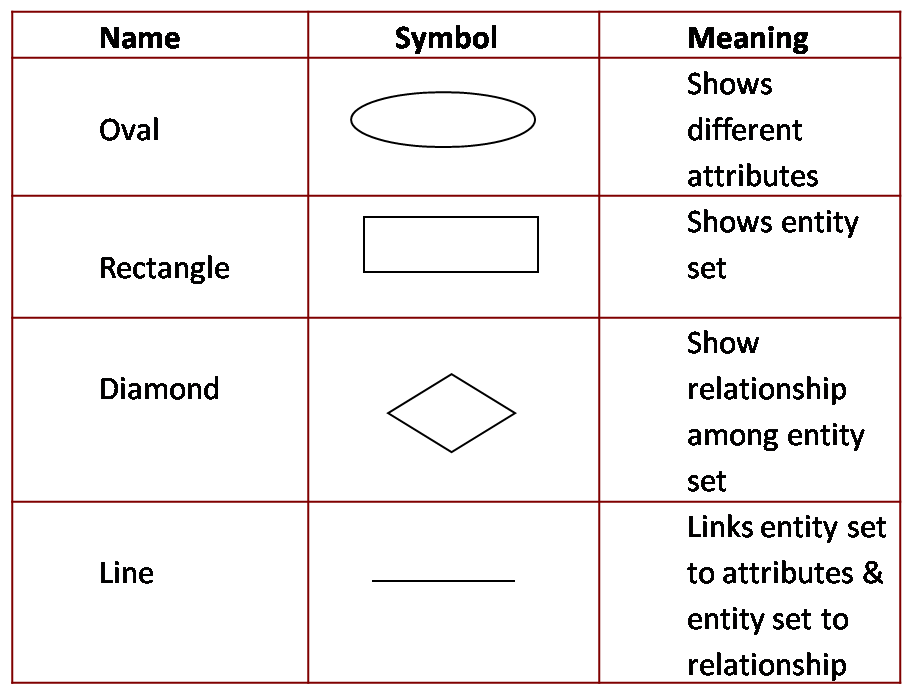
\includegraphics[width=12cm]{ER_Symbol}
	\end{center}
\caption{Symbols Used}
\end{figure}


\begin{figure}[!h]
	\begin{center}
		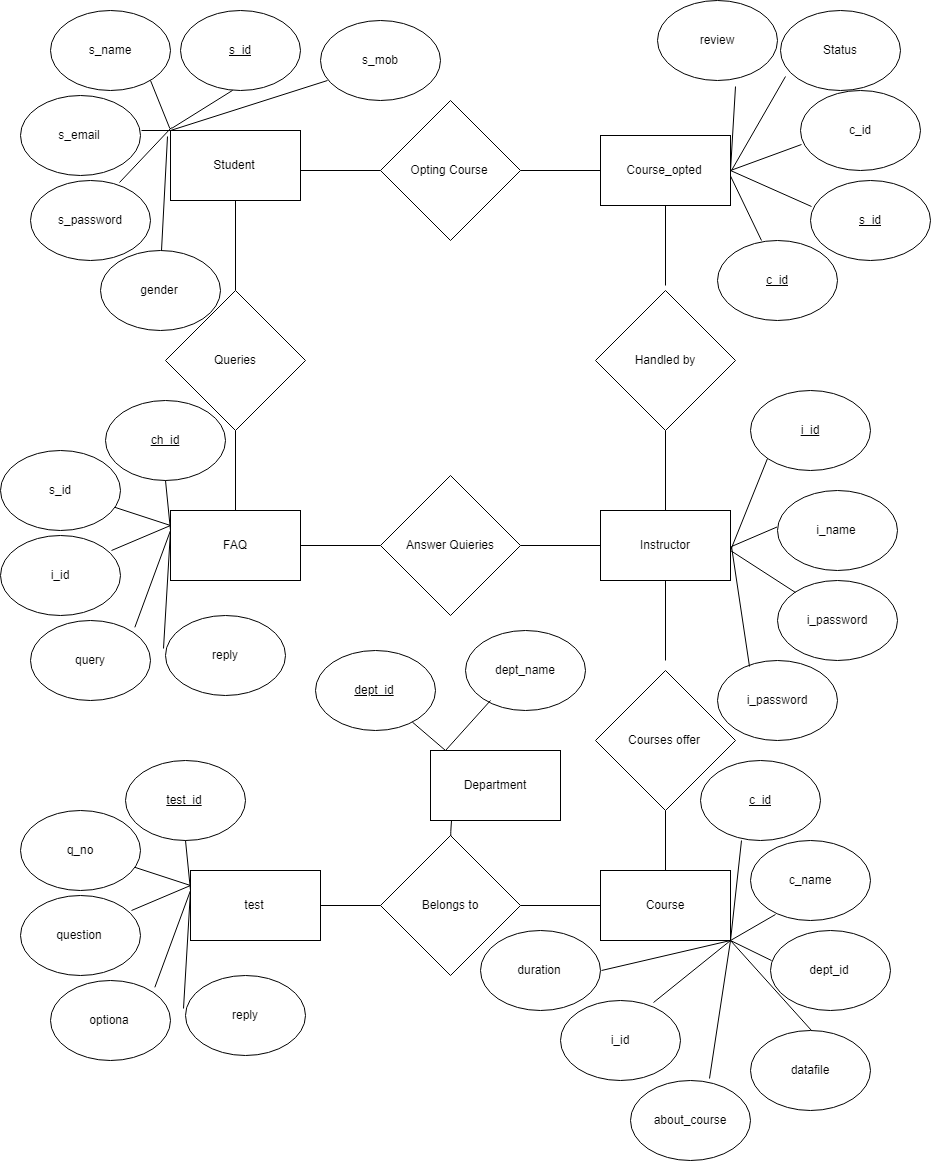
\includegraphics[height=20cm]{ERdiagram.png}
	\end{center}
\caption{ER Diagram}
\end{figure}
%
%\subsubsection{Use Case/UML Diagrams}
%
\section{Sprint Details}
%
\renewcommand{\arraystretch}{1.25}
\begin{center}
\begin{tabular}{|c|p{4cm}|c|c|c|}
\hline
{\bf Task Name	} & {\bf Description} & {\bf Priority}	& {\bf Status} & {\bf 	Durations (Days)}\\
\hline
Sprint 1 & Requirement Collection and UI Design    &  High     &  Completed  &	 17\\
\hline
Task 1   &	Data Collection  &  High     &  Completed  &  1\\
\hline
Task 2	 & Database Design   &  Medium	&  Completed  &	 2\\
\hline
Task 3	 & UI Design    &  Medium   &  Completed  &	14\\
\hline
Sprint 2	 & Adding sections     &  Medium	&  Completed  &  20\\
\hline
Task 1	 & Admin secton    &  Medium	&  Complete   &  8\\
\hline
Task 2  	 & Instructor section	  &  High	    &  Completed  &  8\\
\hline
Task 3   	& Student  section	  &   Medium	&  Completed  & 4\\
\hline
\end{tabular}
\end{center}
\renewcommand{\arraystretch}{1}
%
\section{Details of daily scrum meeting}
%
Daily scrum meetings were held on each day of a sprint. The meetings were held in the office premises of the team at 9:30 am. These scrum meetings were strictly time-boxed to 15 minutes. This was to keep the discussion brisk but relevant.

All team members were required to attend scrum meetings. Since both the Scrum Master and product owner are committed team members, they are expected to attend and participate. Anyone else was allowed to attend, but was there only to listen. This made scrum meetings an excellent way for a Scrum team to disseminate information.

The daily scrum meeting was not used as a problem-solving or issue resolution meeting. Issues that were raised were taken off-line and usually dealt with by the relevant subgroup immediately after the meeting. During the daily scrum, each team member answered the following three questions:
\begin{itemize}
\item
    What did you do yesterday?
\item
    What will you do today?
\item
    Are there any impediments in your way?
\end{itemize}

By focusing on what each person accomplished on a day and would accomplish the next day, the team would gain an excellent understanding of what work had been done and what work remained. The daily scrum meeting was not a status update meeting in which a boss was collecting information about who was behind schedule. Rather, it was a  meeting in which team members made commitments to each other.
%
\section{Details of bi-weekly meeting}
%
%
\renewcommand{\arraystretch}{1.25}
\begin{center}
\begin{tabular}{|p{2cm}|p{2.5cm}|p{8cm}|}
\hline
{\bf Bi-weekly Meeting No.} & {\bf Date} & {\bf Details} \\
\hline
Bi-weekly Meeting 1 & 18-03-2019 & Requirement Collection and Database Design \\
\hline
Bi-weekly Meeting 2 & 01-04-2019 & UI Design  \\
\hline
Bi-weekly Meeting 3 & 15-04-2019 & Admin section \\
\hline
Bi-weekly Meeting 4 & 30-04-2019 & Instructor and Student sections \\
\hline
\end{tabular}
\end{center}
\renewcommand{\arraystretch}{1}
%
%
%   *********************  APPENDIX  ***********************
%
%
\chapter{VERSIONING}
%
%
\renewcommand{\arraystretch}{1.25}
\begin{center}
\begin{tabular}{|p{3cm}|p{5cm}|}
\hline
{\bf Sprint Number} & {\bf Current Version Number}\\
\hline
Sprint 1 & V1 \\
\hline
Sprint 2 & V2 \\  
\hline
\end{tabular}
\end{center}
\renewcommand{\arraystretch}{1}
%
%   *********************  APPENDIX ***********************
%
\chapter{DATA FLOW DIAGRAMS}
Data flow is the one of the best ways of documenting the entire functionality of the system. For the system, which will have some data flows in and have some processing inside and then some data flow out from the system can be documented or represented effectively by means of data flow diagrams. 

The data flow diagrams are a diagrammatic representation of the system, which has input, process and outputs. Once any system is represented using a data flow diagrams we can identify the following things easily: 
\begin{enumerate}
\item Various entities interacting with the system are identified
\item Flow of data from one entity to another is identified
\item The various processes involved in between the interaction of two or more entities in the system are clearly pointed out.  
\item The various data stores, which hold the data in between the processes, are clearly identified.
\end{enumerate}

\begin{figure}[!h]
	\begin{center}
		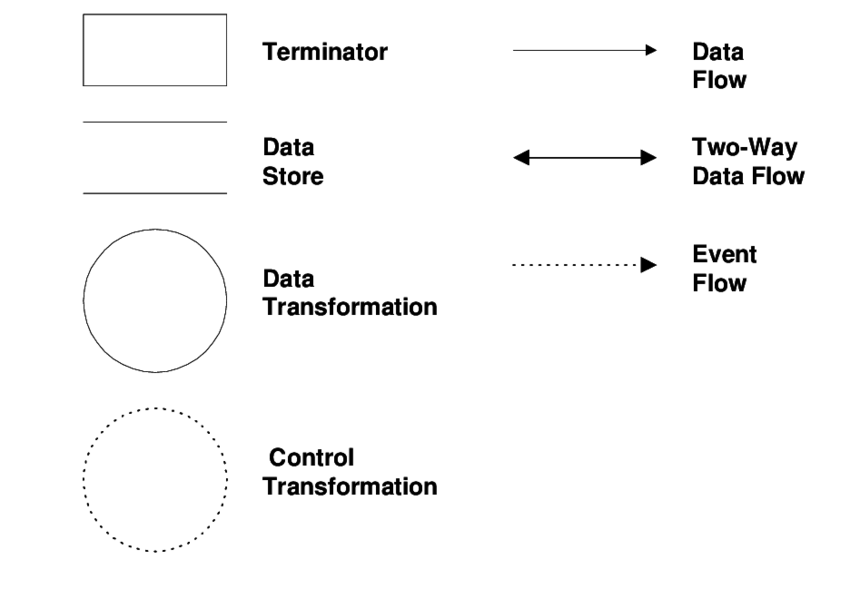
\includegraphics[width=12cm]{DFD_Symbols}
	\end{center}
\caption{DFD Symbols}
\end{figure}


\begin{figure}
  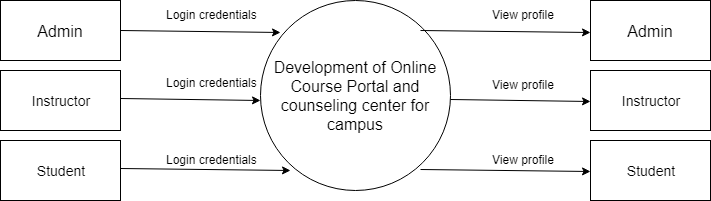
\includegraphics[width=\linewidth]{DFDlevel0.png}
  \caption{ Level 0}
  \label{fig1:Data Flow Diagram Level 0}
\end{figure}

\begin{figure}
  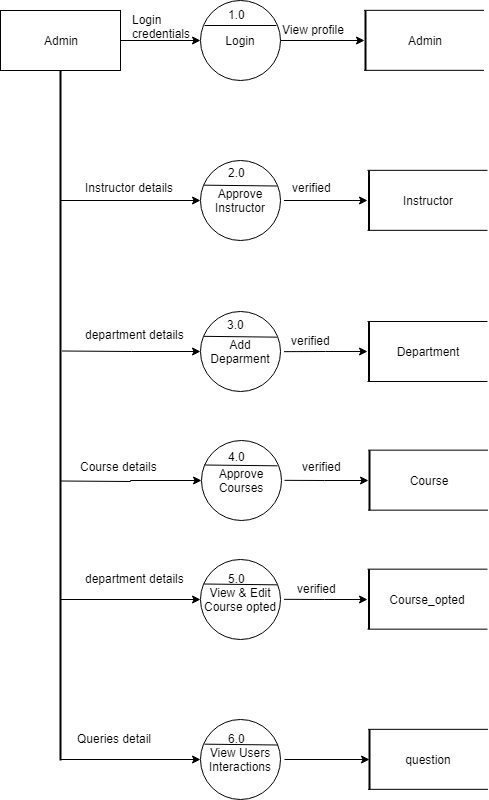
\includegraphics[height=20cm]{level1dfdAdmin.png}
  \caption{Level 1 Admin}
  \label{fig1:Data Flow Diagram Level 1 : Admin}
\end{figure}

\begin{figure}
  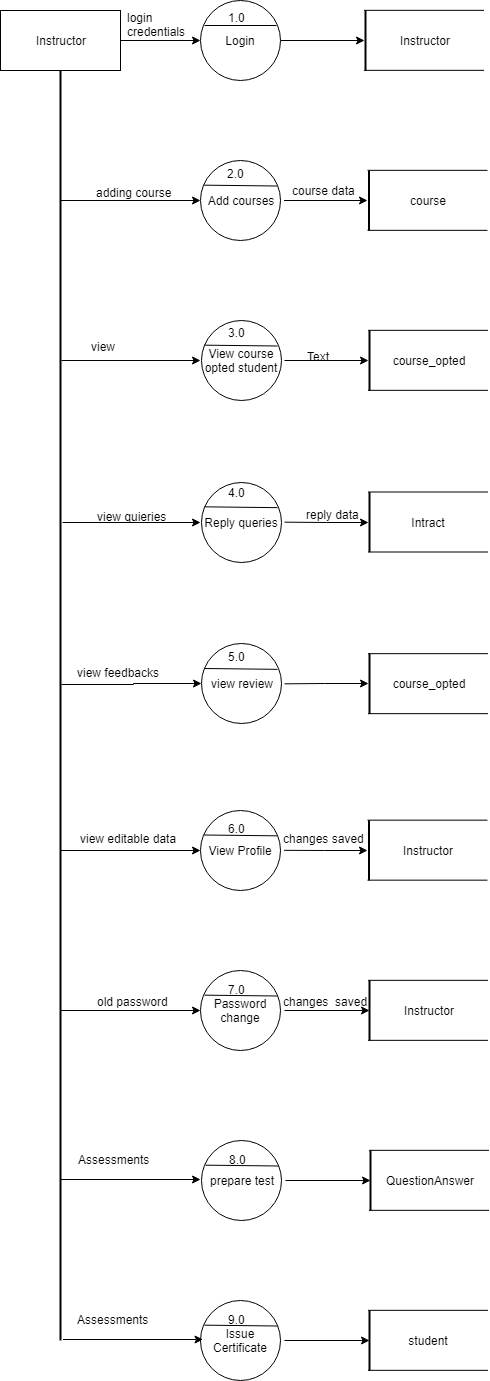
\includegraphics[height=20cm,width=12cm]{dfdlevel1Instructor.png}
  \caption{ Level 1 Instructor}
  \label{fig1:Data Flow Diagram Level 1 : Instructor}
\end{figure}

\begin{figure}
  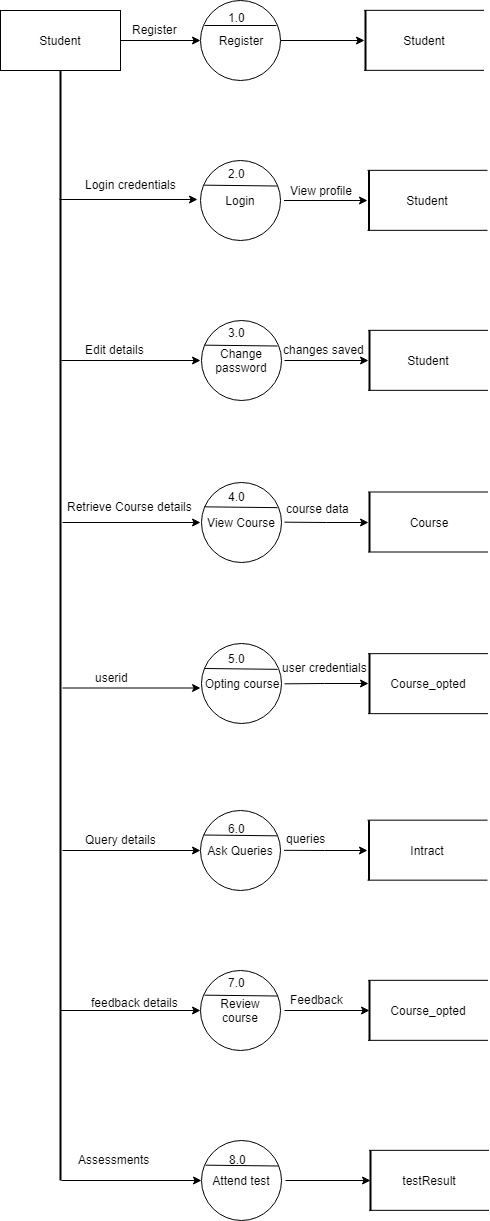
\includegraphics[height=20cm,width=12cm]{StudentDFDlevel1.png}
  \caption{ Level 1 Student}
  \label{fig1:Data Flow Diagram Level 1 : Student}
\end{figure}
%
%
%   *********************  APPENDIX ***********************
%
\chapter{TABLE STRUCTURE}
\begin{table}[!h]
Table Name    :    {\bf admin}\\
Description      :  To store the details of admin


\begin{tabular}{|l|l|l|l|}
\hline
{\bf sl }&{ \bf Name}&{ \bf Type}  &{ \bf Attributes} \\ 
\hline
1  & a\_id       & int(5)      & PRIMARY KEY \\ 
\hline
2  & a\_name     & varchar(30) &    NOT NULL         \\ 
\hline
3  & a\_email    & varchar(30) &    NOT NULL         \\ 
\hline
4  & a\_password & varchar(10) &      NOT NULL       \\ 
\hline
\end{tabular}
\caption{Admin table}
\end{table}


\begin{table}[!h]
Table Name    :    {\bf student}\\
Description      :  To store the details of student


\begin{tabular}{|l|l|l|l|}
\hline
\bf sl.no & \bf Name        & \bf Type        & \bf Attributes  \\ 
\hline
1     & s\_id       & int(5)      & PRIMARY KEY \\ 
\hline
2     & s\_name     & varchar(15) &      NOT NULL       \\ 
\hline
3     & gender      & varchar(6)  &      NOT NULL       \\ 
\hline
4     & s\_mob      & varchar(10) &     NOT NULL        \\ 
\hline
5     & s\_email    & varchar(25) &       NOT NULL      \\ 
\hline
6     & s\_password & varchar(15) &    NOT NULL         \\ 
\hline
\end{tabular}
\caption{Student table}
\end{table}

\begin{table}[!h]
Table Name    :    {\bf Instructor}\\
Description      :  To store the details of Instructor


\begin{tabular}{|l|l|l|l|}
\hline
\bf sl.no & \bf Name        & \bf Type        & \bf Constrains  \\ 
\hline
1     & i\_id       & int(5)      & PRIMARY KEY \\ 
\hline
2     & i\_name     & varchar(15) &  NOT NULL       \\ 
\hline
3     & gender      & varchar(6)  &      NOT NULL  \\ 
\hline
4     & i\_mob      & varchar(10) &    NOT NULL         \\ 
\hline
5     & i\_email    & varchar(25) &      NOT NULL       \\ 
\hline
6     & i\_password & varchar(15) &    NOT NULL         \\ 
\hline
7     & institution & varchar(25) &      NOT NULL       \\ 
\hline
8     & workaddress & varchar(25) &  NOT NULL           \\ 
\hline
9     & status      & varchar(10) &       NOT NULL      \\ 
\hline
\end{tabular}
\caption{Instructor table}
\end{table}

\begin{table}[!h]
Table Name    :    {\bf course}\\
Description      :  To store the details of courses


\begin{tabular}{|l|l|l|l|}
\hline
\bf sl.no & \bf Name          & \bf Type         & \bf Constrains  \\ 
\hline
1     & c\_id         & int(5)       & PRIMARY KEY \\ 
\hline
2     & c\_name       & varchar(15)  &    NOT NULL  \\ 
\hline
3     & about\_course & varchar(250) &  NOT NULL     \\ 
\hline
4     & i\_id         & int(10)      &       NOT NULL      \\ 
\hline
5     & duration      & varchar(10)  &     NOT NULL        \\ 
\hline
6     & dept          & varchar(20)  &       NOT NULL      \\ 
\hline
7     & datafile      & varchar(250) &    NOT NULL         \\ 
\hline
\end{tabular}
\caption{Course table}
\end{table}

\begin{table}[!h]
Table Name    :    {\bf courseopted}\\
Description      :  To store the details of course opted students


\begin{tabular}{|l|l|l|l|}
\hline
\bf sl.no & \bf Name   & \bf Type         & \bf Constrains  \\ 
\hline
1     & co\_id & int(5)       & PRIMARY KEY \\
 \hline
2     & s\_id  & varchar(10)  &       NOT NULL      \\ 
\hline
3     & review & varchar(250) &     NULL        \\ 
\hline
4     & c\_id  & int(5)       &    NOT NULL         \\ 
\hline
5     & status & varchar(10)  &    NOT NULL         \\ 
\hline
\end{tabular}
\caption{CourseOpted table}
\end{table}

\begin{table}[!h]
Table Name    :    {\bf dept}\\
Description      :  To store the details of departments


\begin{tabular}{|l|l|l|l|}
\hline
\bf sl.no & \bf Name       & \bf Type        & \bf Constrains  \\ 
\hline
1     & dept\_id   & int(5)      & PRIMARY KEY \\ 
\hline
2     & dept\_name & varchar(20) &      NOT NULL       \\ 
\hline
\end{tabular}
\caption{Department table}
\end{table}

\begin{table}[!h]
Table Name    :    {\bf test}\\
Description      :  To store the details of question paper


\begin{tabular}{|l|l|l|l|}
\hline
\bf sl.no & \bf Name     & \bf Type         & \bf Constrains  \\ 
\hline
1     & test\_id & int(5)       & PRIMARY KEY \\ 
\hline
2     & c\_id    & int(5)       &       NOT NULL      \\ 
\hline
3     & q\_no    & int(5)       &          NOT NULL   \\ 
\hline
4     & Question & varchar(250) &    NOT NULL         \\ 
\hline
5     & oa       & varchar(250) &        NOT NULL     \\ 
\hline
6     & ob       & varchar(250) &      NOT NULL       \\ 
\hline
7     & oc       & varchar(250) &      NOT NULL       \\ 
\hline
8     & od       & varchar(250) &        NOT NULL     \\ 
\hline
9     & answer   & varchar(250) &       NOT NULL      \\ 
\hline
\end{tabular}
\caption{Test table}
\end{table}

\begin{table}[!h]
Table Name    :    {\bf result}\\
Description      :  To store the details of result of students


\begin{tabular}{|l|l|l|l|}
\hline
\bf sl.no &  \bf Name   &\bf  Type   &\bf Constrains  \\ 
\hline
1     & tr\_id & int(5) & PRIMARY KEY \\ 
\hline
2     & s\_id  & int(5) &       NOT NULL      \\ 
\hline
3     & c\_id  & int(5) &       NOT NULL      \\ 
\hline
4     & score  & int(5) &      NOT NULL       \\ 
\hline
\end{tabular}
\caption{Result table}
\end{table}

\begin{table}[!h]
Table Name    :    {\bf question}\\
Description      :  To store the details of queries of students


\begin{tabular}{|l|l|l|l|}
\hline
 \bf sl.no & \bf  Name     & \bf  Type         & \bf Constrains  \\ 
\hline
1     & q\_id    & int(5)       & PRIMARY KEY \\ 
\hline
2     & s\_id    & int(5)       &    NOT NULL         \\
\hline
3     & question & varchar(500) &    NOT NULL         \\ 
\hline
\end{tabular}
\caption{Queries table}
\end{table}

\begin{table}[!h]
Table Name    :    {\bf answer}\\
Description      :  To store the details of replay to queries.


\begin{tabular}{|l|l|l|l|}
\hline
\bf sl.no & \bf Name    & \bf Type         & \bf Constrains  \\ 
\hline
1     & ans\_id & int(5)       & PRIMARY KEY \\ 
\hline
2     & i\_id   & int(5)       &        NOT NULL     \\ 
\hline
3     & q\_id   & varchar(6)   &     NOT NULL        \\ 
\hline
4     & answer  & varchar(500) & NOT NULL            \\ 
\hline
\end{tabular}
\caption{Replay table}
\end{table}

%
%
%   *********************  APPENDIX ***********************
%
\chapter{SAMPLE SCREENSHOTS}
%
\begin{figure}[!h]
	\begin{center}
		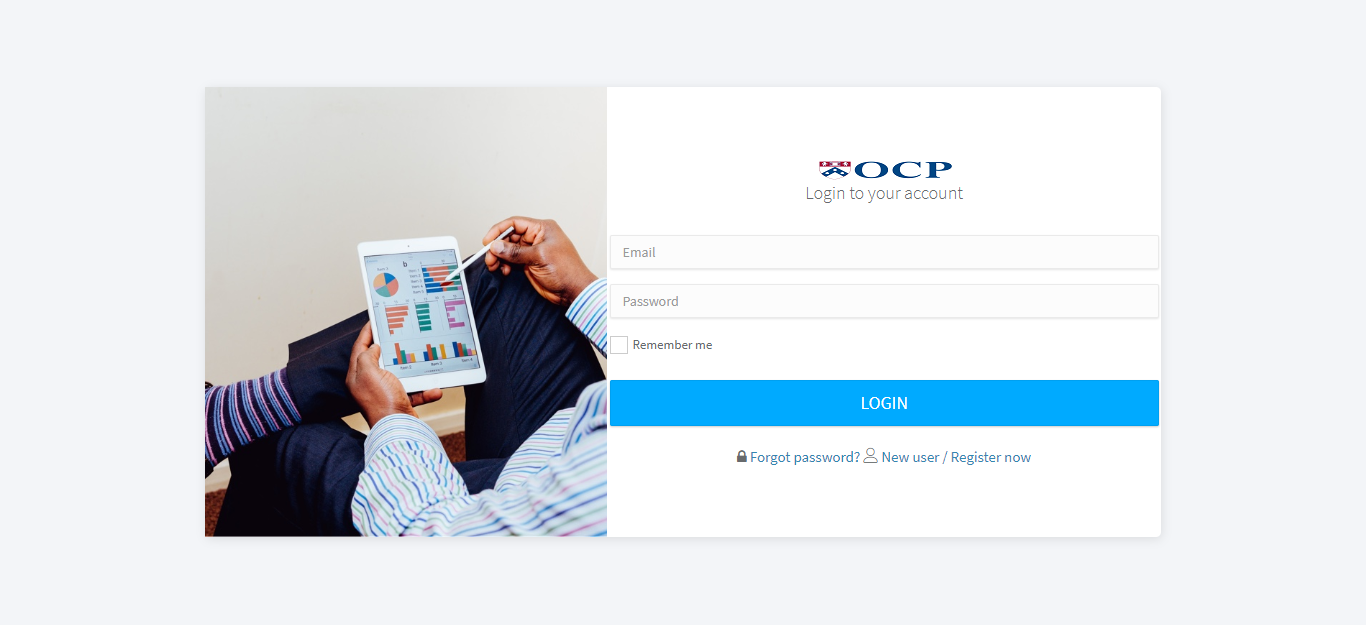
\includegraphics[height=9cm,width=15cm]{login.png}
	\end{center}
\caption{Login Page}
\end{figure}

\begin{figure}[!h]
	\begin{center}
		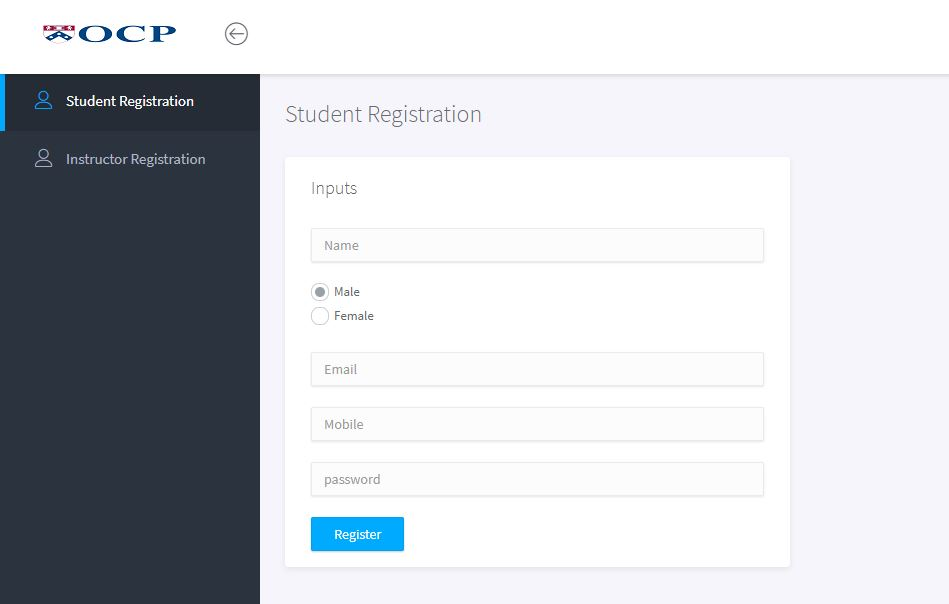
\includegraphics[height=9cm]{studentreg.jpg}
	\end{center}
\caption{Student registration Page}
\end{figure}

\begin{figure}[!h]
	\begin{center}
		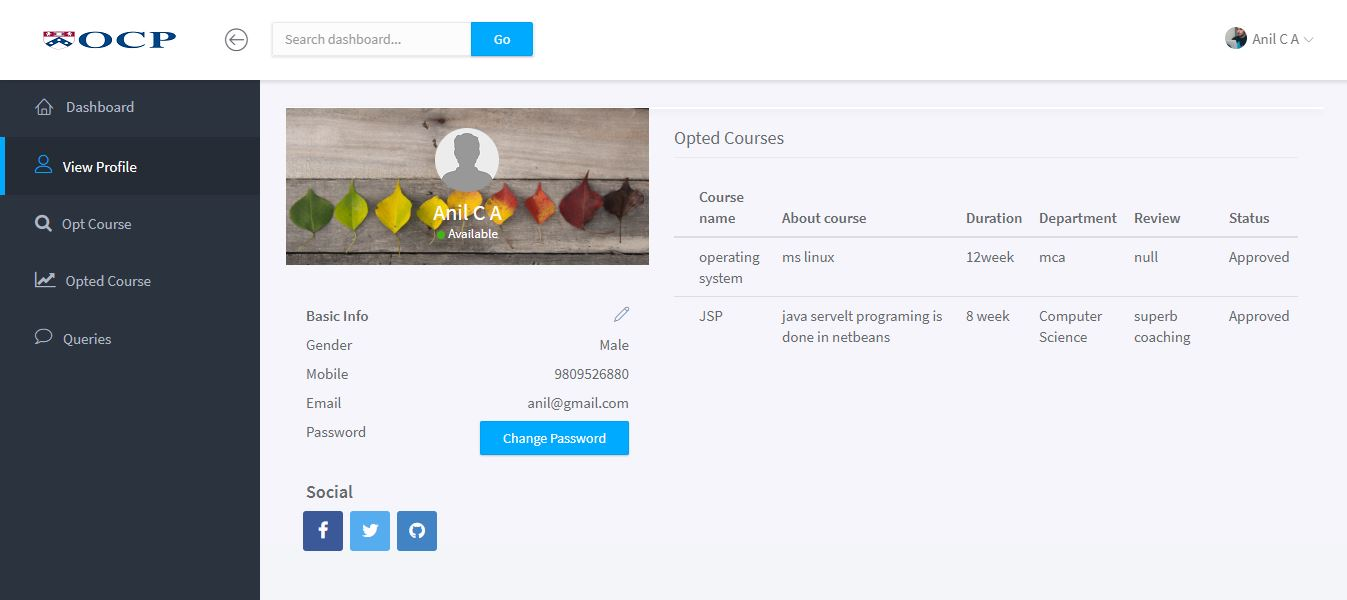
\includegraphics[height=9cm,width=15cm]{studentprofile.jpg}
	\end{center}
\caption{Student profile Page}
\end{figure}

\begin{figure}[!h]
	\begin{center}
		\includegraphics[height=9cm,width=15cm]{instructorreg.jpg}
	\end{center}
\caption{Instructor registration Page}
\end{figure}

\begin{figure}[!h]
	\begin{center}
		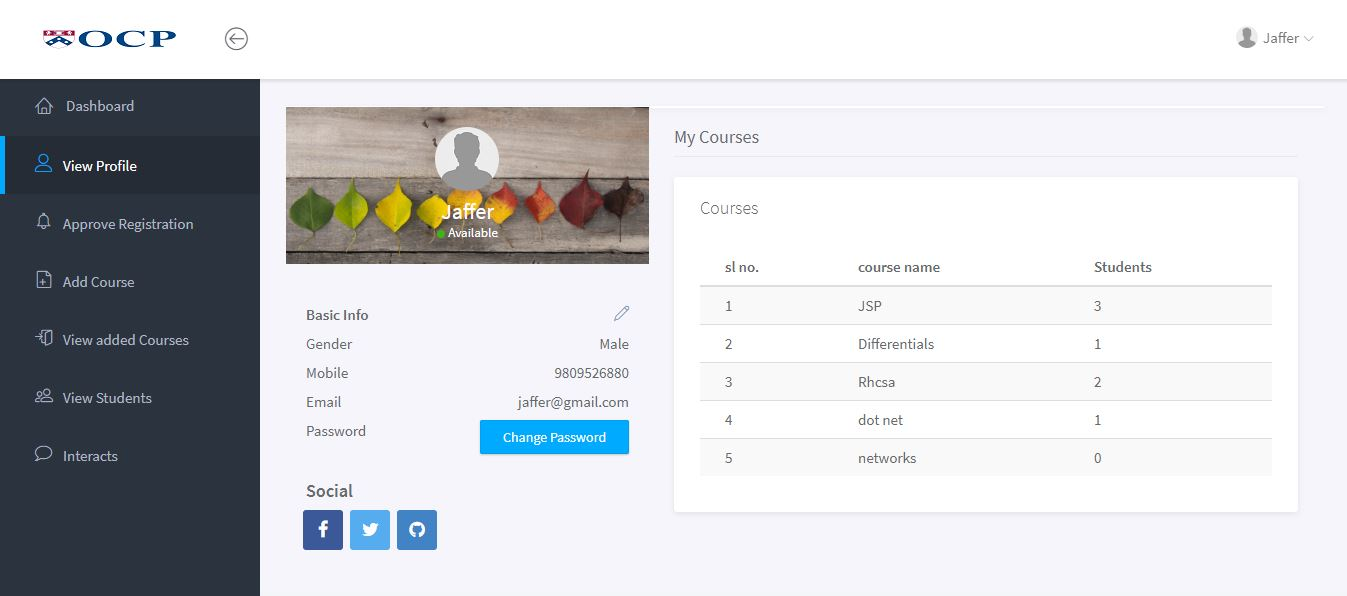
\includegraphics[height=9cm,width=15cm]{instructorprofile.jpg}
	\end{center}
\caption{Instructor Profile Page}
\end{figure}

\begin{figure}[!h]
	\begin{center}
		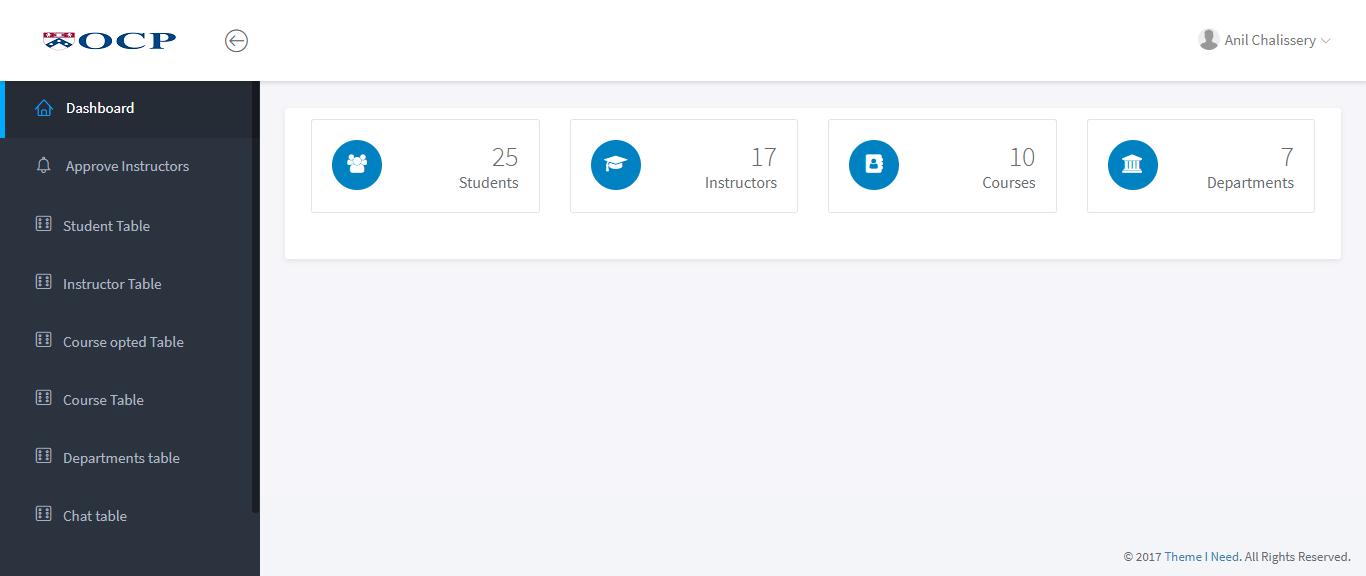
\includegraphics[height=9cm,width=16cm]{adminpanel.png}
	\end{center}
\caption{Admin panel Page}
\end{figure}

\begin{figure}[!h]
	\begin{center}
		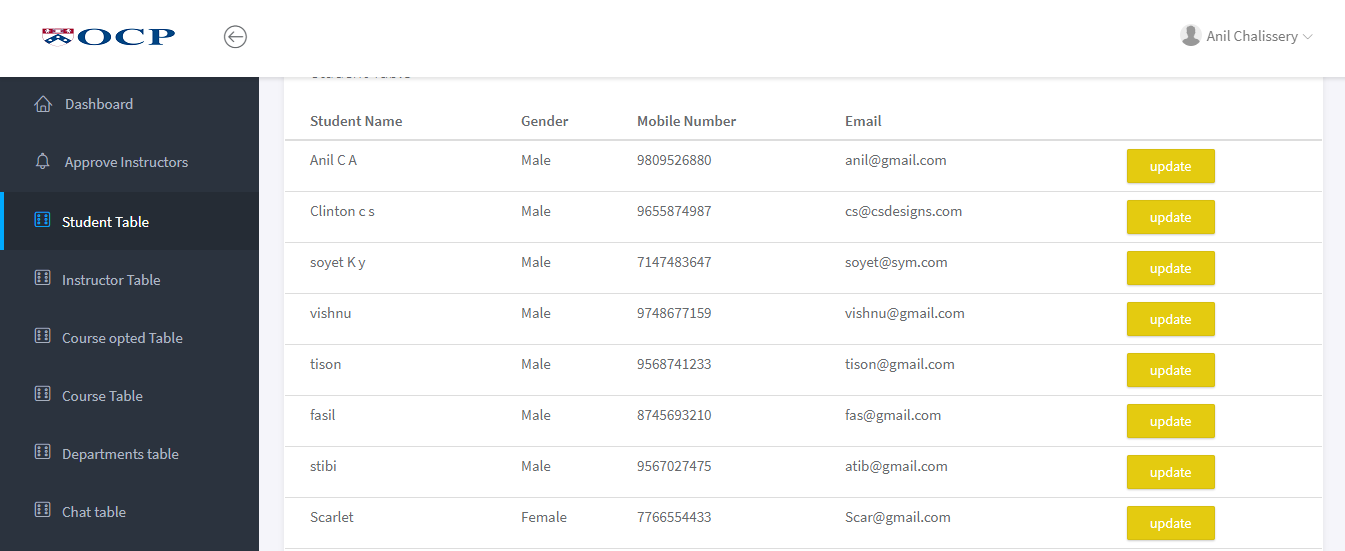
\includegraphics[height=9cm,width=16cm]{studentstable.png}
	\end{center}
\caption{Students data Page}
\end{figure}

\begin{figure}[!h]
	\begin{center}
		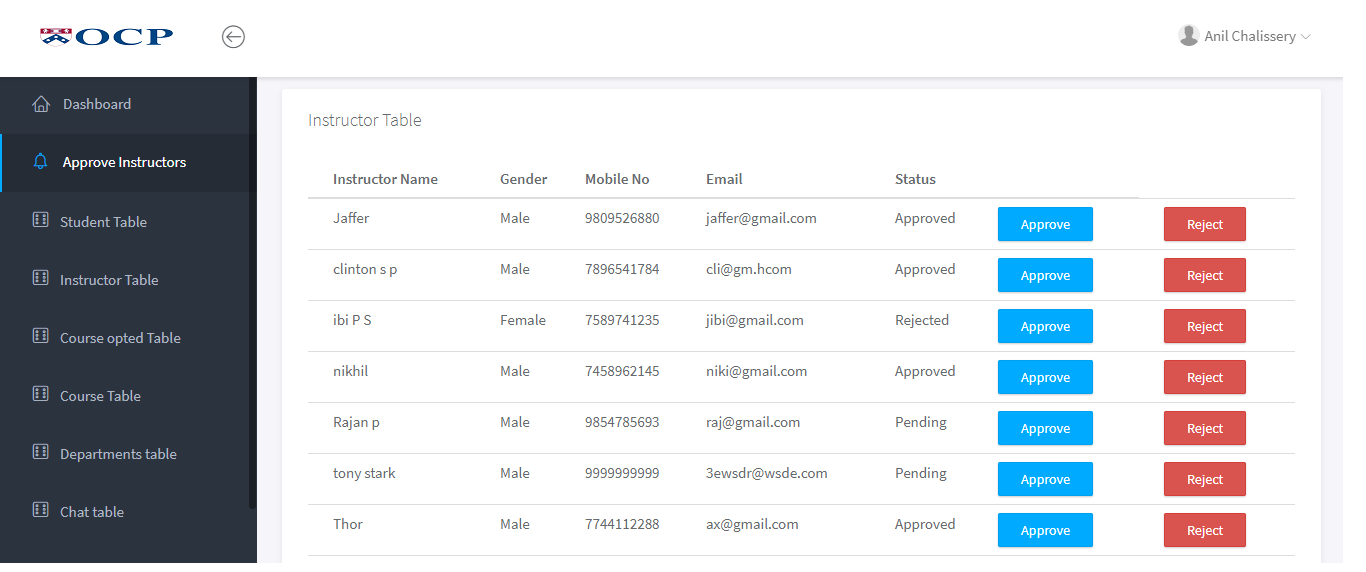
\includegraphics[width=16cm,height=9cm]{approveInstructor.png}
	\end{center}
\caption{Approving Instructor Page}
\end{figure}

\begin{figure}[!h]
	\begin{center}
		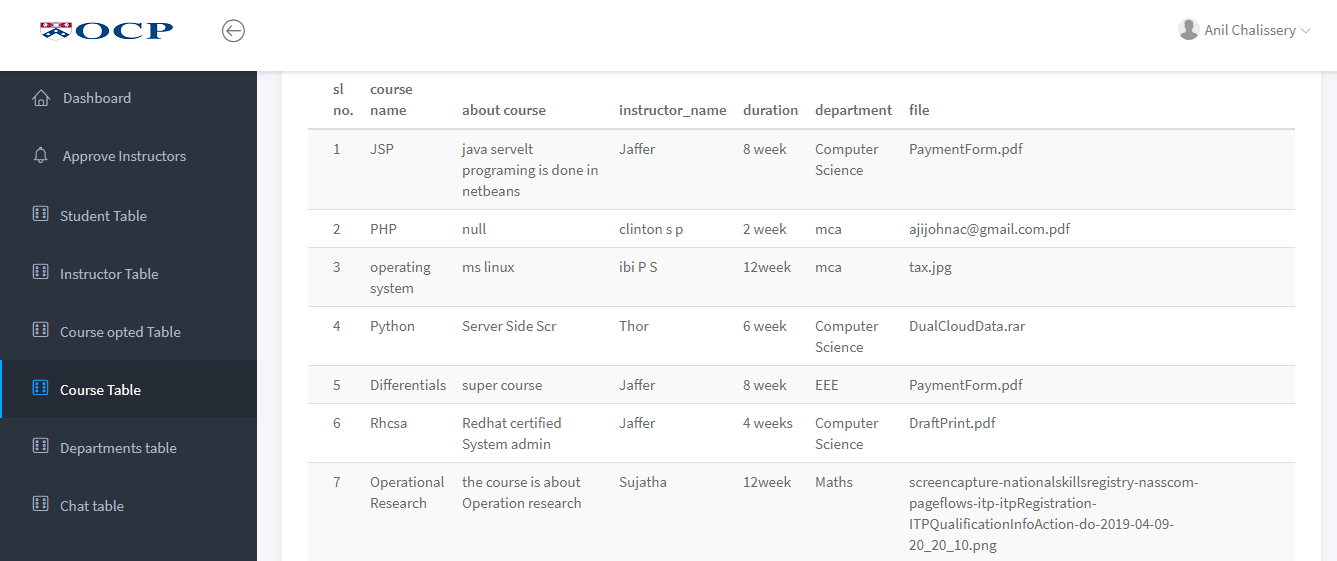
\includegraphics[width=16cm,height=9cm]{coursedata.png}
	\end{center}
\caption{ Course data Page}
\end{figure}

\begin{figure}[!h]
	\begin{center}
		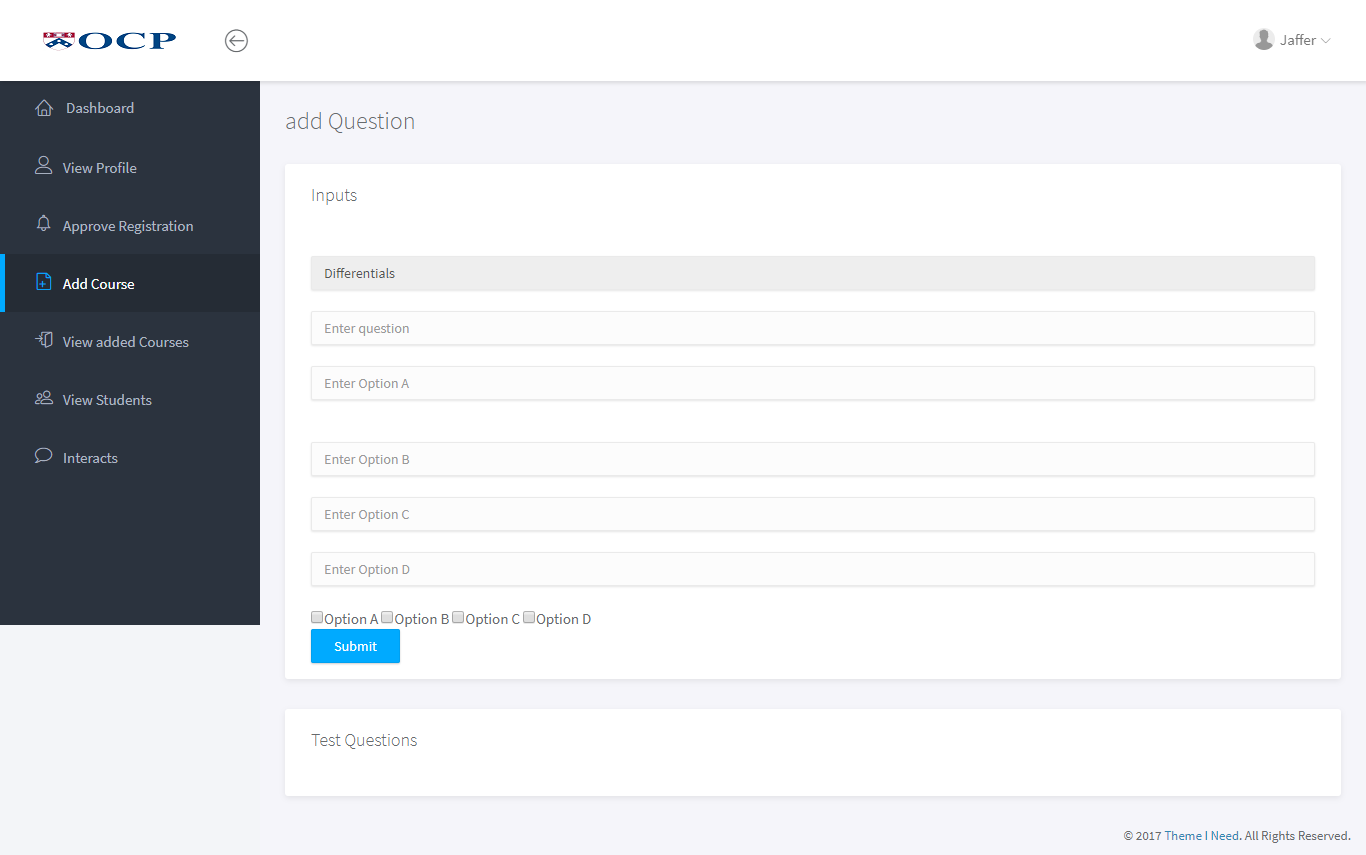
\includegraphics[width=15cm,height=12cm]{addTest.png}
	\end{center}
\caption{Adding test page}
\end{figure}

\begin{figure}[!h]
	\begin{center}
		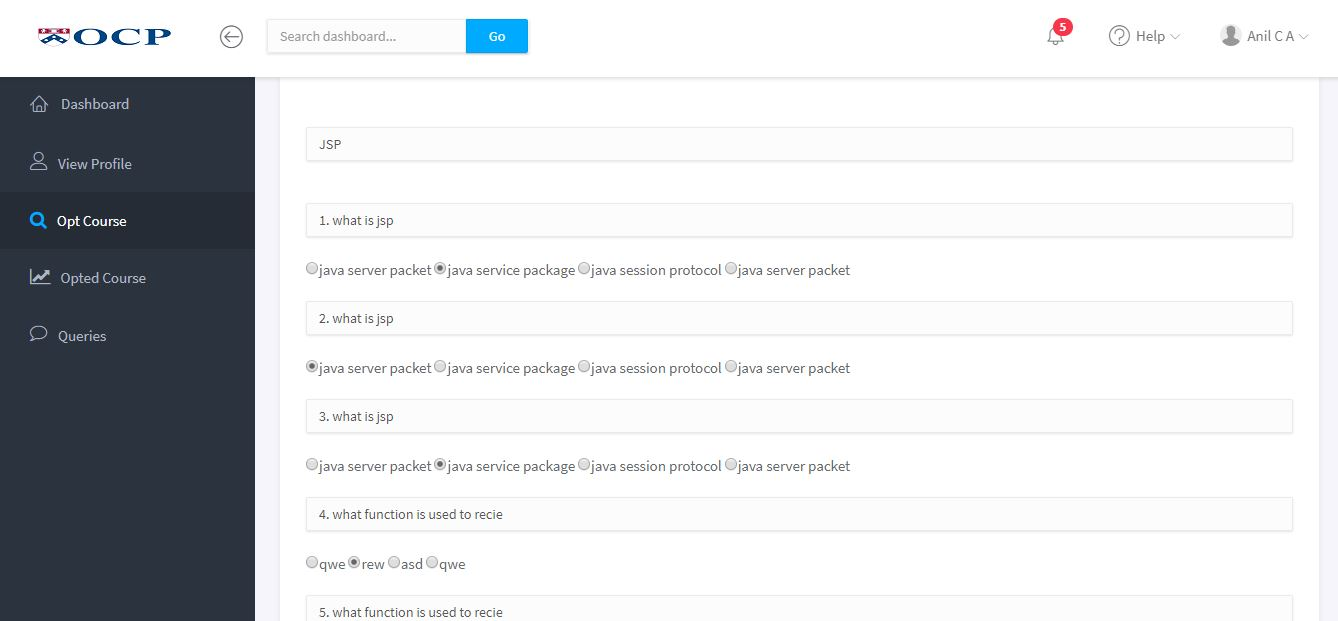
\includegraphics[width=15cm,height=10cm]{test.jpg}
	\end{center}
\caption{Attending test page}
\end{figure}

\begin{figure}[!h]
	\begin{center}
		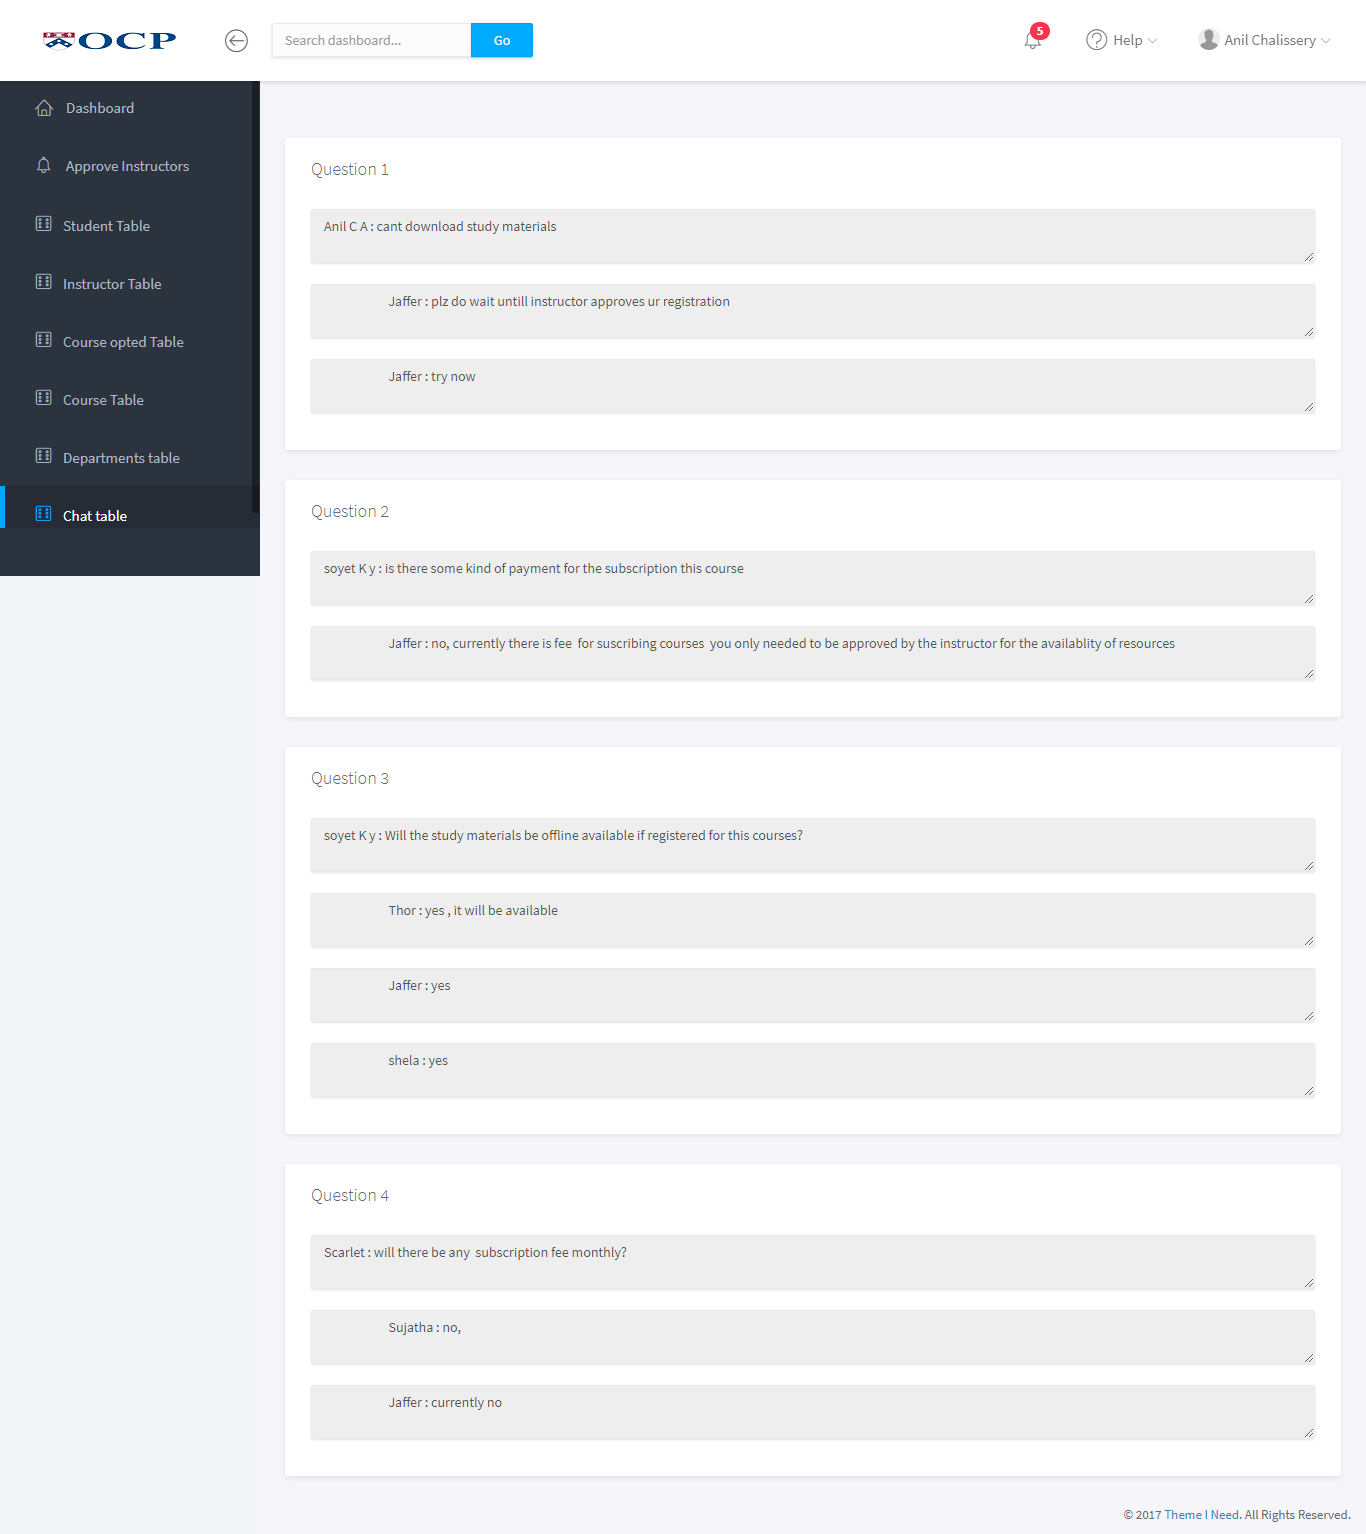
\includegraphics[width=17cm,height=15cm]{FAQ}
	\end{center}
\caption{FAQ Page}
\end{figure}



%
%   *********************  APPENDIX ***********************
%
%\chapter{REPORTS}
%
% *****************************************************
%
% ***   Creating Bibliography   ***
%
% Do not delete the following two lines
%
\clearpage
\addcontentsline{toc}{chapter}{Bibliography}
%
%   The markups for creating the bibliography 
%   begins here. Do not change the two lines 
%   "\begin{thebibliography}{99}" and 
%   "\end{thebibliography}".
%   One sample bibliography item is included. 
%   Each new item is to be preceded by
%   "\bibitem{itemx}".
%   Add additional items if there are any.
%   Bibliography styles:
%   Titles of books   : Italics  {use {\em Title} )
%   URLs of websites  : Type-writer (use {\tt Title} )
%   Titles of papers  : In double quotes (use ``Title")
%
\begin{thebibliography}{99}
%
\bibitem{item1}
{\em First Lessons in \LaTeX}, by Dr. V N Krishnachandran, 
Vidya Academy of Science \& Technology, 
Thrissur - 680 501, 2011.
\bibitem{item2}
{www.w3schools.com}
\bibitem{item3}{https://www.tutorialspoint.com/jsp/}
\bibitem{item4}{https://www.javatpoint.com/jsp-tutorial}

\bibitem{item5}{http://www.mysqltutorial.org/}
\bibitem{item6}{https://netbeans.org/kb/docs/java/quickstart.html}


%
\end{thebibliography}
%
%
%   Printing the last page
%
%
\newpage
\thispagestyle{empty}
\vspace*{\fill}
\begin{flushright}

\includegraphics{VidyaLogo.JPG}\\[0.5cm]
{\Large \bf \sf  Department of \vdept\ }\\
{\sf Vidya Academy of Science \& Technology\\
Thalakkottukara, Thrissur - 680 501\\
({\tt http://www.vidyaacademy.ac.in})}
\end{flushright}
%
%
%
%   ***   The end   ***
%
%
\end{document}